\documentclass[letterpaper,12pt]{article}
\usepackage{tabularx} % extra features for tabular environment
\usepackage{amsmath}  % improve math presentation
\usepackage{amsfonts}
\usepackage{verbatim}
\usepackage{graphicx} % takes care of graphic including machinery
\usepackage[margin=1in,letterpaper]{geometry} % decreases margins
\usepackage{cite} % takes care of citations
\usepackage[final]{hyperref} % adds hyper links inside the generated pdf file
\hypersetup{
	colorlinks=true,       % false: boxed links; true: colored links
	linkcolor=blue,        % color of internal links
	citecolor=blue,        % color of links to bibliography
	filecolor=magenta,     % color of file links
	urlcolor=blue         
}
\usepackage{blindtext}

\usepackage{units}
%++++++++++++++++++++++++++++++++++++++++


\begin{document}

\title{Uncertain Effects of DFT Functionals on Charge Mobility Calculations}
\author{authors}
\date{\today}
\maketitle

\begin{abstract}
    We study the uncertainty effect from the DFT functional to the charge mobility calculations of organic semiconductors (OSC). 
    The charge mobilities of the BCP and MADN devices are calculated from the first principle multiscale model. Using a total of 10 different DFT functionals, we find that the electronic structure properties have similar distributions as indicated by Wasserstein distance, while the charge mobility of the BHANDHLYP functional has a large deviation. 
    Further investigation reveals that the BHANDHLYP functional leads to a trap site, and the charge mobility is very sensitive to the trap sites' energy, so a small change in the site's energy results in a large deviation of ToF.  

    We further investigate the uncertainty effect of electronic structure properties on the charge mobility 
    We find that the site energy has the most significant effect on the charge mobility and a confidence level of charge mobility is obtained encoding the maximum amount of uncertainty in electronic structure parameters. 
\end{abstract}

\section{Introduction}
Charge mobility is one of the key quantities of interest for OSC.

Charge conductance is due to electron dynamics, so quantum mechanics and Schr\"odinger equation are essential for the theoretical study of charge mobility. 

Due to the complexity of Schr\"odinger Equation, one alternative theory is the density functional theory (DFT). DFT has two challenges. Firstly, it is computationally impossible to perform electronic structure calculations for the whole OSC device. And secondly, the exchange-correlation potential in DFT has an unknown formula.

The first challenge is overcome by approximating the electron dynamics as transition processes between the localized states, with the transition rates calculated as the temperature-activated bi-molecule transition rates, known as the Marcus rate. 
The second challenge is addressed by utilizing DFT functionals to represent the exchange-correlation potential. 
Those functionals are benchmarked to achieve good consistency with many physical quantities, such as ionization potential, and density of states. 

The influence of the different functionals on ToF calculation is missing. 



\section{Results}
\label{sec:result}
The list of figures:
\begin{itemize}
    \item Heat map of $E(f)$ versus $E(f=PBE0)$. This figure visually shows how energy are affected by different functionals and we can learn which sites have large different energies.
    \item Heat map of $J_{i,j}(f)$ versus $J_{i,j}(f=PBE0)$. This figure visually shows how $J_{i,j}$ are affected by different functionals and we can learn the pairs having very different $J_{i,j}$.
    \item Scatter plot of $\Delta \text{ToF}$ versus Wasserstein distance $W_1 (P_f(E),P_{f'}(E))$, and $\Delta \text{ToF}$ versus $\text{KL}(P_f(E),P_{f'}(E))$. This figure shows the change of $\text{ToF}$ as a result of different energy distributions measured by two commonly used metrics. We can learn that $\Delta \text{ToF}$ can be very large even though the two distributions are close.
    \item Scatter plot of standard graph Laplacian matrix 2nd eigenvalue ratio $\frac{\lambda_{2}}{\lambda'_{2}}$ versus ToF ratio $\frac{\text{ToF}_f}{\text{ToF}_{f'}}$. We can learn that $\frac{\lambda_{2}}{\lambda'_{2}}$ is correlated with the change of ToF, and $\lambda_{2}$ is a metric indicating the change of ToF due to the functionals. 
    \item Distribution (Scatter) of 2nd eigenvector entries for specific functionals. This plot tells how the entries are distributed in one-dimensional space, and if any clusters are formed.
    we can learn that in all functionals, some nodes (such as node66) have very different eigenvector entries than others, indicating that those nodes can be partitioned into clusters.
    \item Scatter plot of K-means clustering partition cost $Z_{2c},Z_{3c}$ versus ToF. This plot tells us that in the case of $Z_{3c}$, large ToF corresponds to small $Z_{3c}$, indicating the large ToF system can be partitioned into three clusters with a small cost. 
    \item Scatter plot show $Z_{2c}$ versus $E_{t}$, and $Z_{2c}$ versus ToF when varying the $E_{t}$ to introduce trap. We can learn that When $E_{t}$ is small, there is a log-linear relationship between $Z_{2c}$ and $E_{t}$, ToF. But when $E_{t}$ is large, both $Z_{2c}$ and ToF remain unchanged. This suggests that when $E_{t}$ is large, the node (node66) is not visited in the random walk and does not contribute to the ToF.
    \item Using symmetrized adjacency matrix $W := \frac{1}{2}(W+W^T)$, scatter plot showing $Z_{2c}$ versus $E_{66}$, and $Z_{2c}$ versus ToF is made. In $Z_{2c}$-$E_{66}$ plot we learn that both large and small $E_{66}$ give small $Z_{2c}$, meaning that this symmetrized graph is able to identify trap nodes and nodes that are rarely visited (anti-trap).
\end{itemize}

\subsection{Distribution Distance and  $\Delta$ToF}
\begin{table}[h]
    \centering
    \begin{tabular}{c c c c c }
    \hline
        functional & scaleHFX & $\lambda_h$ [eV]   & ToF [s]  & $\sigma(E)$ \\ 
        \hline
        PBE0 & 0.25 & 0.388 & 1.23e-3  & 0.175 \\
        PBE & 0 & 0.303  & 1.04e-3  & 0.172 \\ 
        B3LYP & 0.20 & 0.375  & 4.28e-3  & 0.175 \\
        BHANDHLYP & 0.5 & 0.494  &\textbf{737.94}  & 0.192 \\
        TPSS & 0 & 0.310  &1.37e-2 &  0.168 \\
        BP86 & 0 & 0.304  & 7.46e-3 & 0.175 \\
        wB97X & 0.157 & 0.505 & 2.92e-2  & 0.191 \\
        wB97X-D3 & 0.195 & 0.496 & 4.89e-2  & 0.180 \\
        M06L & 0 & 0.312 & 3.19e-1  & 0.165 \\
        BHLYP & 0.5 & 0.493 &  2.47 & 0.192 \\
    \hline
    \end{tabular}
    \caption{ The values of $\lambda_h$, ToF, Stationary state velocity and energy standard deviation of BCP molecules calculated from different functionals. }
    \label{tab:para}
\end{table}
\begin{table}[h]
    \centering
    \begin{tabular}{c c c  }
    \hline
        functional & ToF[s] & $\mu$ [m/s]   \\ 
        \hline
        PBE0 & 2.39e-8 & 5.68e-5 \\
        PBE & 6.03e-9 & 2.25e-4  \\ 
        B3LYP & 1.67e-8 & 8.13e-5 \\
        BHANDHLYP & 3.36e-4 & 4.04e-9   \\
        TPSS & 1.23e-8 & 1.10e-4   \\
        BP86 & 3.77e-7 & 3.59e-6   \\
        wB97X & 1.68e-6 & 8.08e-7  \\
        wB97X-D3 & 6.92e-7 & 1.96e-6  \\
        M06L & 3.90e-3 & 3.47e-10  \\
    \hline
    \end{tabular}
    \caption{ Mobility and ToF with drift electric field $6e7$ V/m. }
    \label{tab:para2}
\end{table}

\begin{figure}
    \centering
    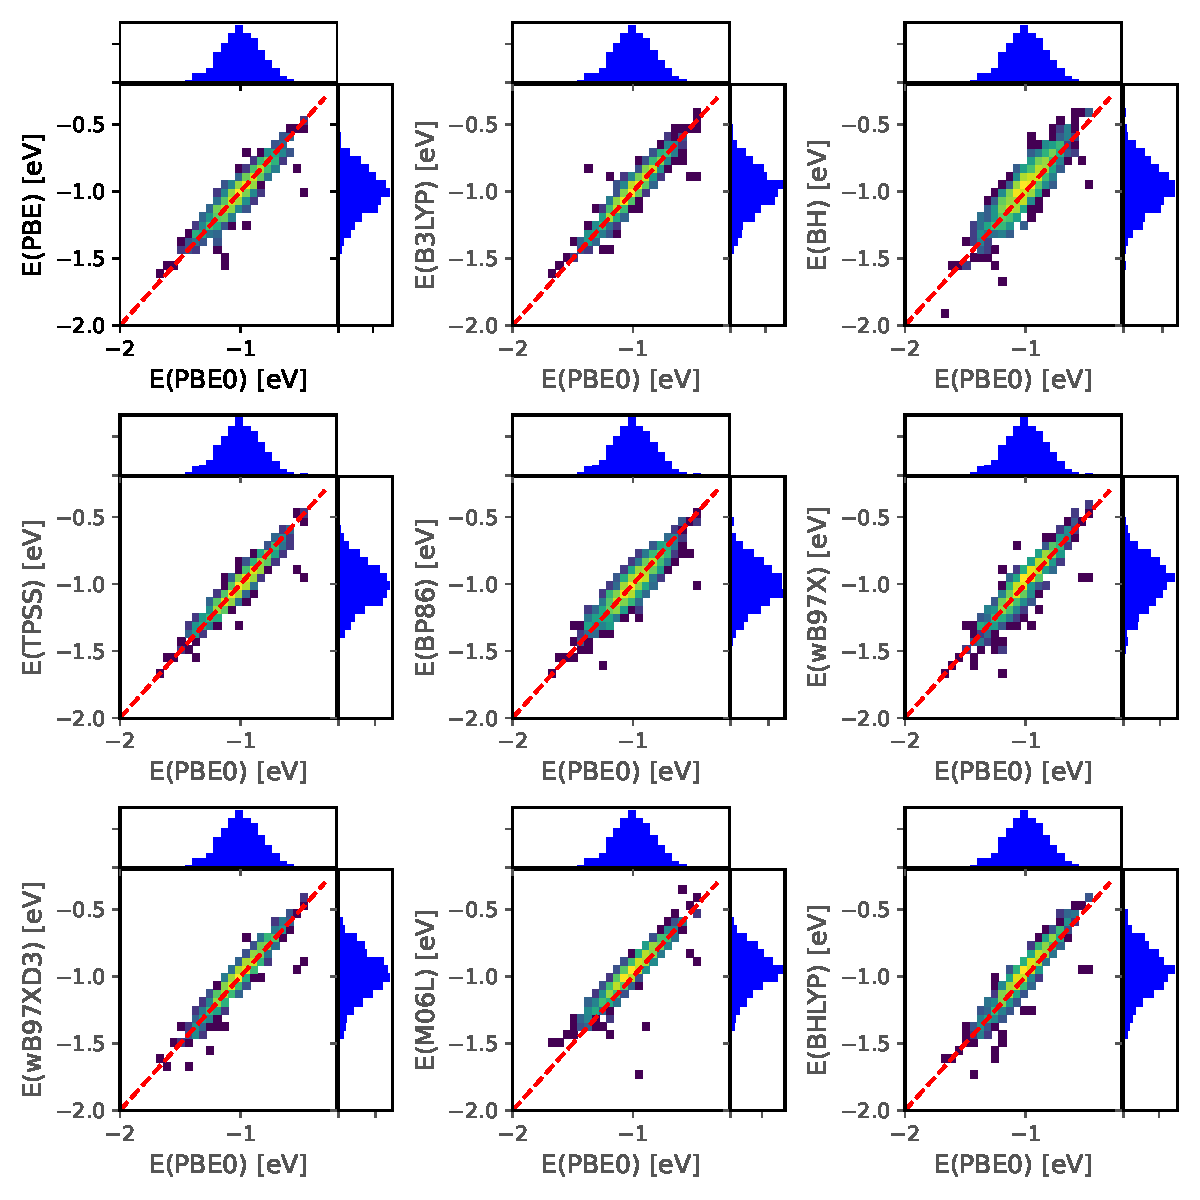
\includegraphics[width=0.95\textwidth]{figs/scatterE_all.pdf}
    \caption{Energy heat maps. $X$-axis the is energy of BCP molecules obtained using $f$=PEB0, the $Y$-axis is the energy from a different functional $f'$ than PBE0.}
    \label{fig:scatterE}
\end{figure}

\begin{figure}
    \centering
    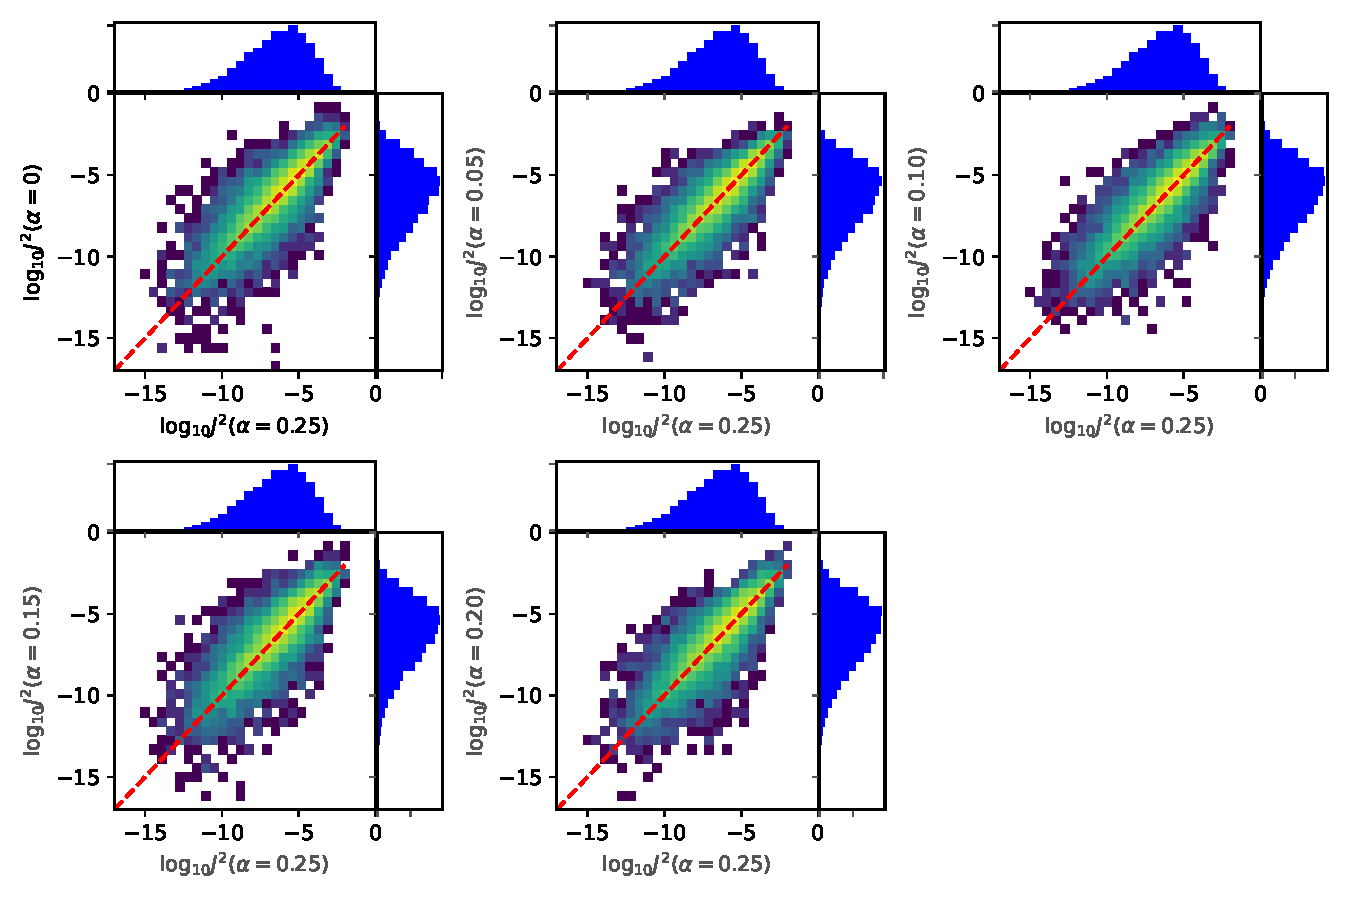
\includegraphics[width=0.95\textwidth]{figs/scatterJ_all.pdf}
    \caption{$\log_{10}(J^2)$ scatter heat maps where $X$-axis the is $\log_{10}(J^2)$ of BCP molecules obtained using $f$=PEB0, the $Y$-axis is the $\log_{10}(J^2)$ from a different functional $f'$ than PBE0.}
    \label{fig:scatterJ}
\end{figure}

First-principle multiscale model for ToF study begins with a set of molecules (molecular structures) and DFT functionals, which characterize the ground state electronic structure of molecules, then a graph is defined, and finally, a ToF is calculated. 

In this multiscale model, the molecular structure is kept fixed while different choices of DFT functionals are made. Using those functionals similar distributions of parameters $E_i,J_{ij}$ are obtained. 
Compared with those parameter distributions, the ToF shows a large difference, especially for $f^\text{BHANDHLYP}$ which gives ToF $\sim 700$ (the level of insulator).

Table \ref{tab:para} summarizes statistical properties: the name of exchange-correlation functionals for DFT calculation, the magnitude of the Hartree-Fock exchange energy (scaleHFX), reorganization energy ($\lambda_h$), time-of-flight (ToF), and energy disorder ($\sigma(E)$) for various functionals. Drift ToF and mobility at an electric field of $6 \times 10^7$ V/m are presented in Table \ref{tab:para2}.

As is shown in Table \ref{tab:para}, the energy disorders $\sigma_E$ are in a small range from 0.165 to 0.192 eV.

Scatter plots comparing the site energies ($E_i$) and coupling elements ($J_{i,j}$) of PBE0 functional ($f$=PBE0) with of other functionals ($f'$) are displayed in Figs.\ref{fig:scatterE} and \ref{fig:scatterJ}  respectively.
Figure \ref{fig:scatterE} shows almost all energies obtained from $f=\text{PBE0}$ are very close to energies from other functionals. 
Although a few points stay some distance away from the diagonal, the majority of the scatter points lie on the diagonal line indicating similarity between $E(f^\text{DET})$ for $f^\text{DET} \neq \text{PBE0}$ and $E(\text{PBE0})$.



To further confirm this observation and understand the effect of parameter difference such as energy $\{ E_i \}$ in ToF, the Wasserstein distance ($W_1$) and Kullback-Leibler divergence $KL(P_f(E),P_{f'}(E))$ between two any two energy distributions $w_1(P_f(E),P_{f'}(E))$ are calculated, and plotted against the different in ToF $\Delta $ToF. 
The results are shown in Fig. \ref{fig:distance_ToF}. 
Notably, $W_1(P_f(E),P_{f'}(E))$ and $KL(P_f(E),P_{f'}(E))$ exhibit small variations, contrasting with the large changes observed in $\Delta \text{ToF}$.

Specifically, those figure shows that $W_1(P_f(E),P_{f'}(E))$ and $KL(P_f(E),P_{f'}(E))$ are in a small range, but $\Delta \text{ToF}$ can change significantly. This means $P_f(E)$ does not change a lot with different functionals but the resulting $\Delta \text{ToF}$ change significantly.

Furthermore, the Wasserstein distances of other distributions (such as $P(\Delta E), P(e^{\Delta E})$ shown in Appendix Fig.\ref{fig:distance_ToF}) are not correlated to $\Delta$ToF.

In conclusion, the distribution distance between the parameters themselves can not explain the $\Delta \text{ToF}$. 

\begin{figure}
    \centering
    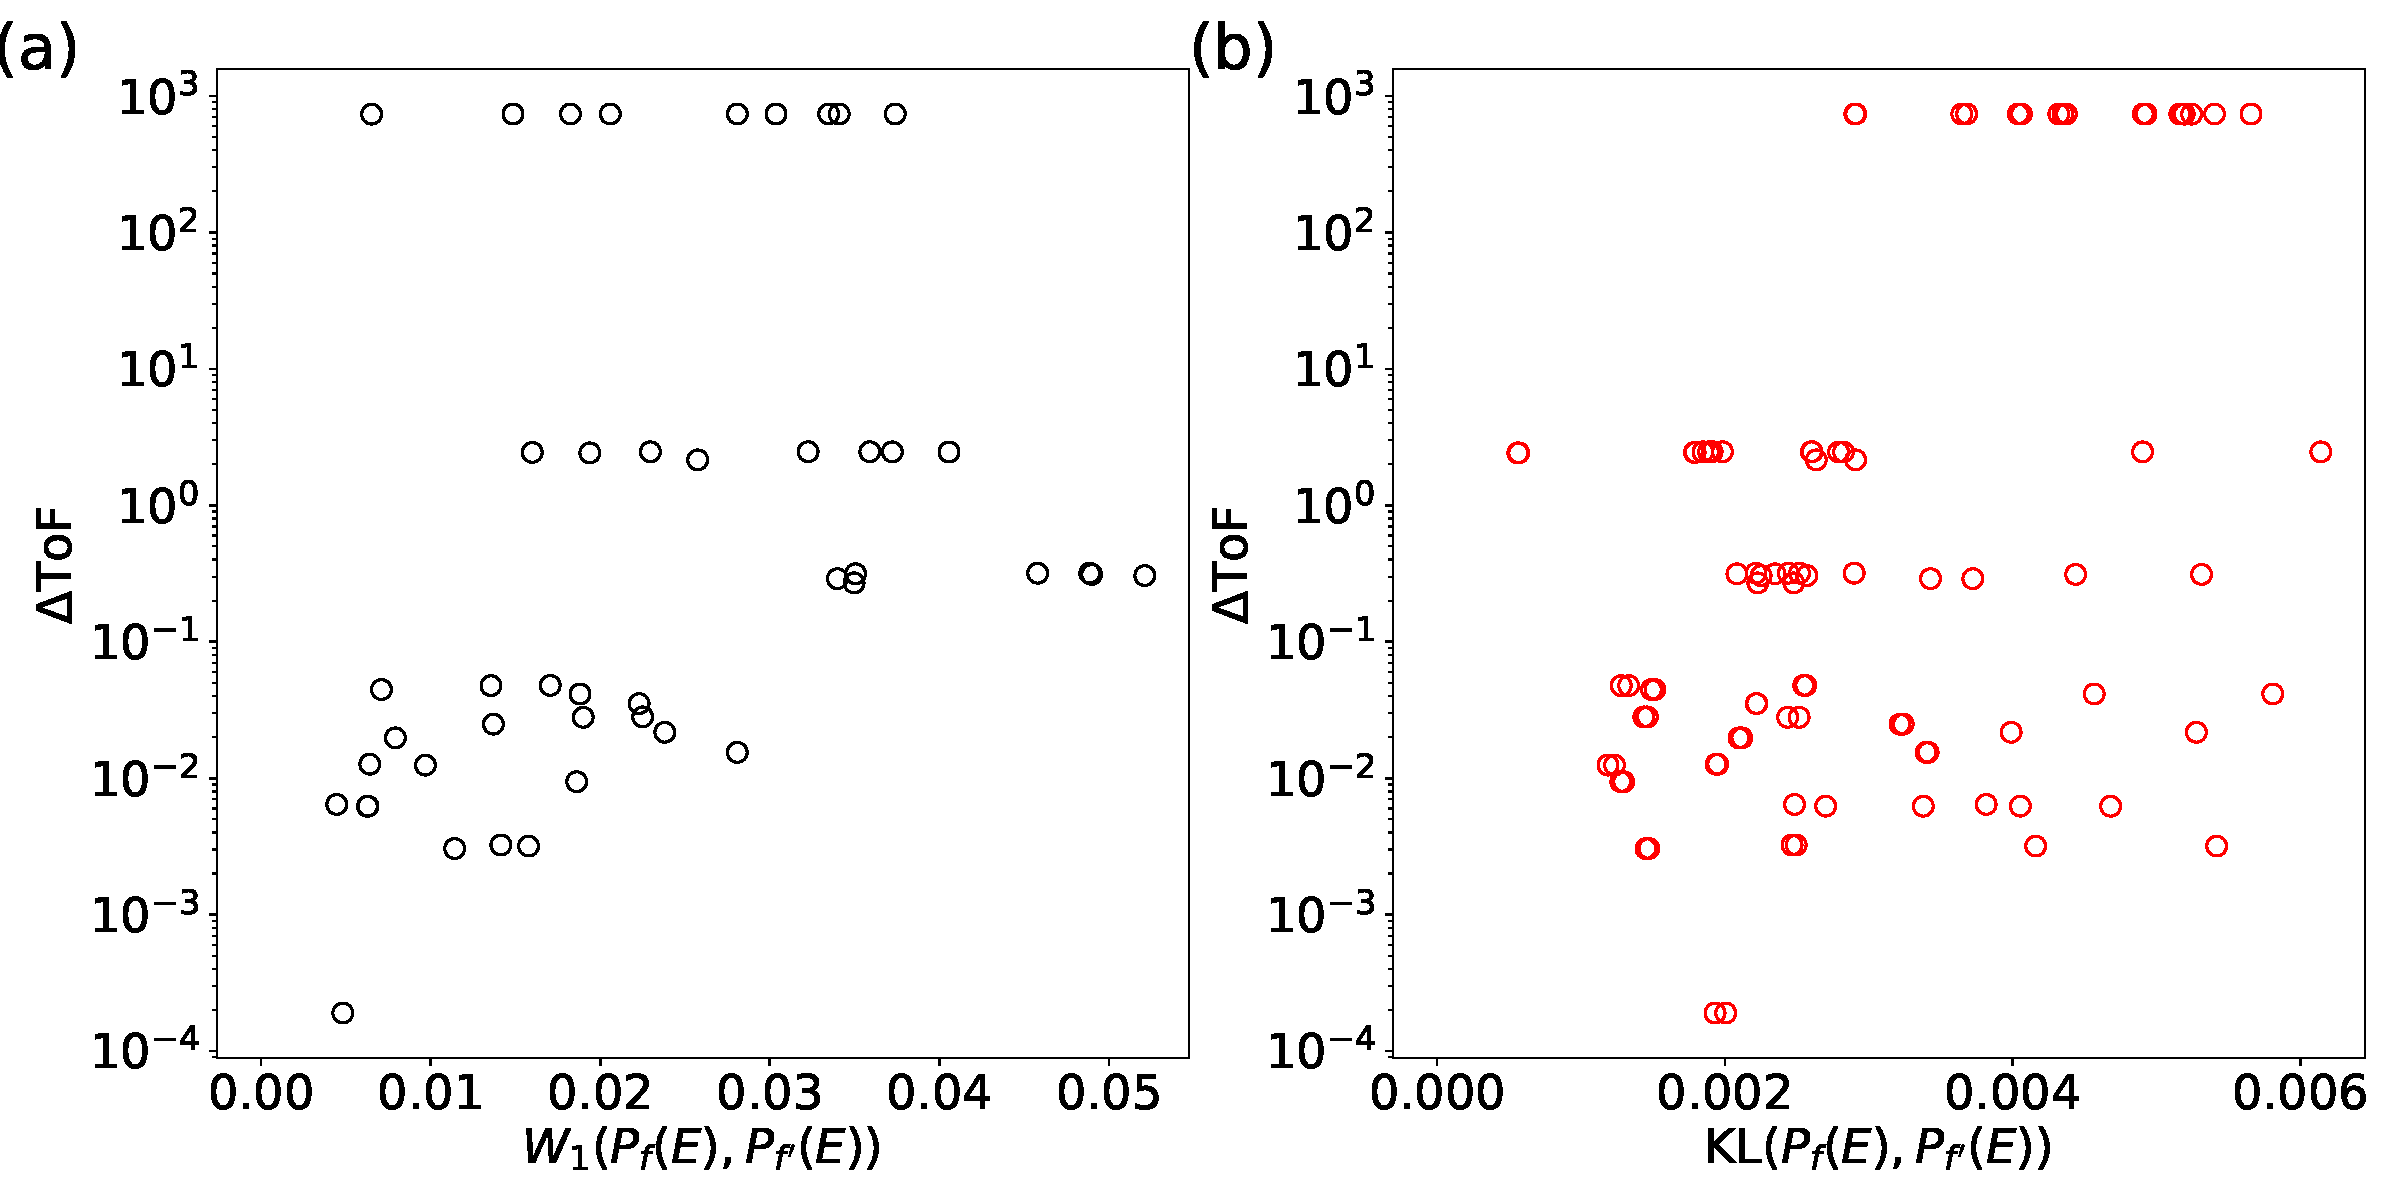
\includegraphics[width=0.9\textwidth]{figs/DeltaToF_W_KL_E.pdf}
    \caption{Left: scatter plot of $W_1(P_f,P_{f'})$ vs. $\Delta \text{ToF}$. 
    Right: scatter plot of  $KL(P_f(E),P_{f'}(E))$ vs. $\Delta \text{ToF}$. }
    \label{fig:distance_ToF}
\end{figure}

\subsection{Spectral Clustering}
The Wasserstein distance metric was found to be ineffective for measuring differences between graph properties. In spectral clustering theory, the second eigenvalue indicates a graph's ability to be partitioned into two clusters. Mapping the graph into a vector $\vec{x} \in \mathbb{R}^n$ with $||\vec{x}||_1=0$ allows partitioning such that nodes in different clusters are maximally separated. This second eigenvalue metric measures the minimum distance between the two most separated clusters, as shown in Equations \ref{eq:min2} and \ref{eq:min3}.

Figure \ref{fig:d_eig_tof} plots $\frac{\text{ToF}(f)}{\text{ToF}(f')}$ against $\frac{\lambda_2(f)}{\lambda_2(f')}$, showing a strong correlation as indicated by the Spearman rank coefficient.
\begin{table}[h]
    \centering
    \begin{tabular}{c c c  }
    \hline
        data set & Spearman rank coefficient & $p$-value   \\ 
        \hline
        $\frac{\lambda_{2,L_W}(f)}{\lambda_{2,L_W}(f')}$ vs $\frac{\text{ToF}(f)}{\text{ToF}(f')}$,  & -0.57 & 4.6e-5 \\
        $\frac{\lambda_{2,L_\text{rw}}(f)}{\lambda_{2,L_\text{rw}}(f')}$ vs $\frac{\text{ToF}(f)}{\text{ToF}(f')}$ & -0.38 & 9.4e-3  \\ 
    \hline
    \end{tabular}
    \caption{ Spearman rank coefficient of relationship between $\frac{\lambda_2(f)}{\lambda_2(f')}$ and  $\frac{\text{ToF}(f)}{\text{ToF}(f')}$}
    \label{tab:spearman}
\end{table}



\begin{figure}
    \centering
    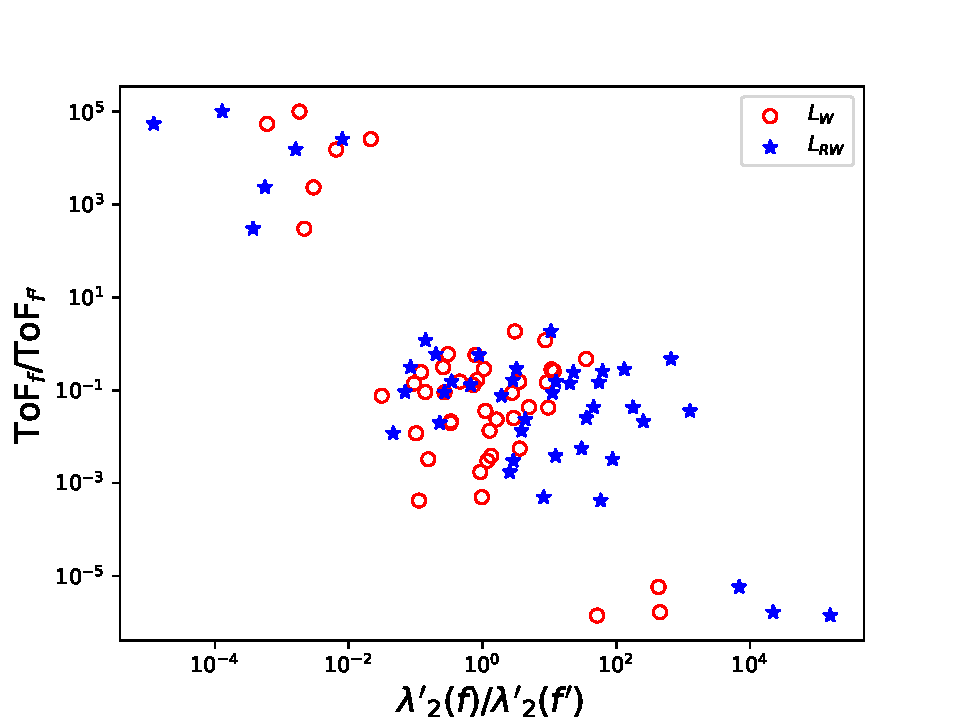
\includegraphics[width=0.6\textwidth]{figs/ratio_tof_2ndEigval.pdf}
    \caption{Scatter plot of $\frac{\lambda_{2}(f)}{\lambda_{2}(f')}$ vs. $\frac{\text{ToF}(f)}{\text{ToF}(f')}$. The type of the Laplacian matrixes is indicated by the legend.}
    \label{fig:d_eig_tof}
\end{figure}

When the graph $G$ is mapped to the space of the second eigenvalue of $L_w$, $\vec{v}_2$,
The equality is obtained in Eqn.\ref{eq:min2}. So the entries of this vector can be used to partition the graph into clusters. The distribution of $\vec{v}_2$ entries are displayed in Fig.\ref{fig:2ndVecLW} and \ref{fig:2ndVecRW}.

\begin{figure}
    \centering
    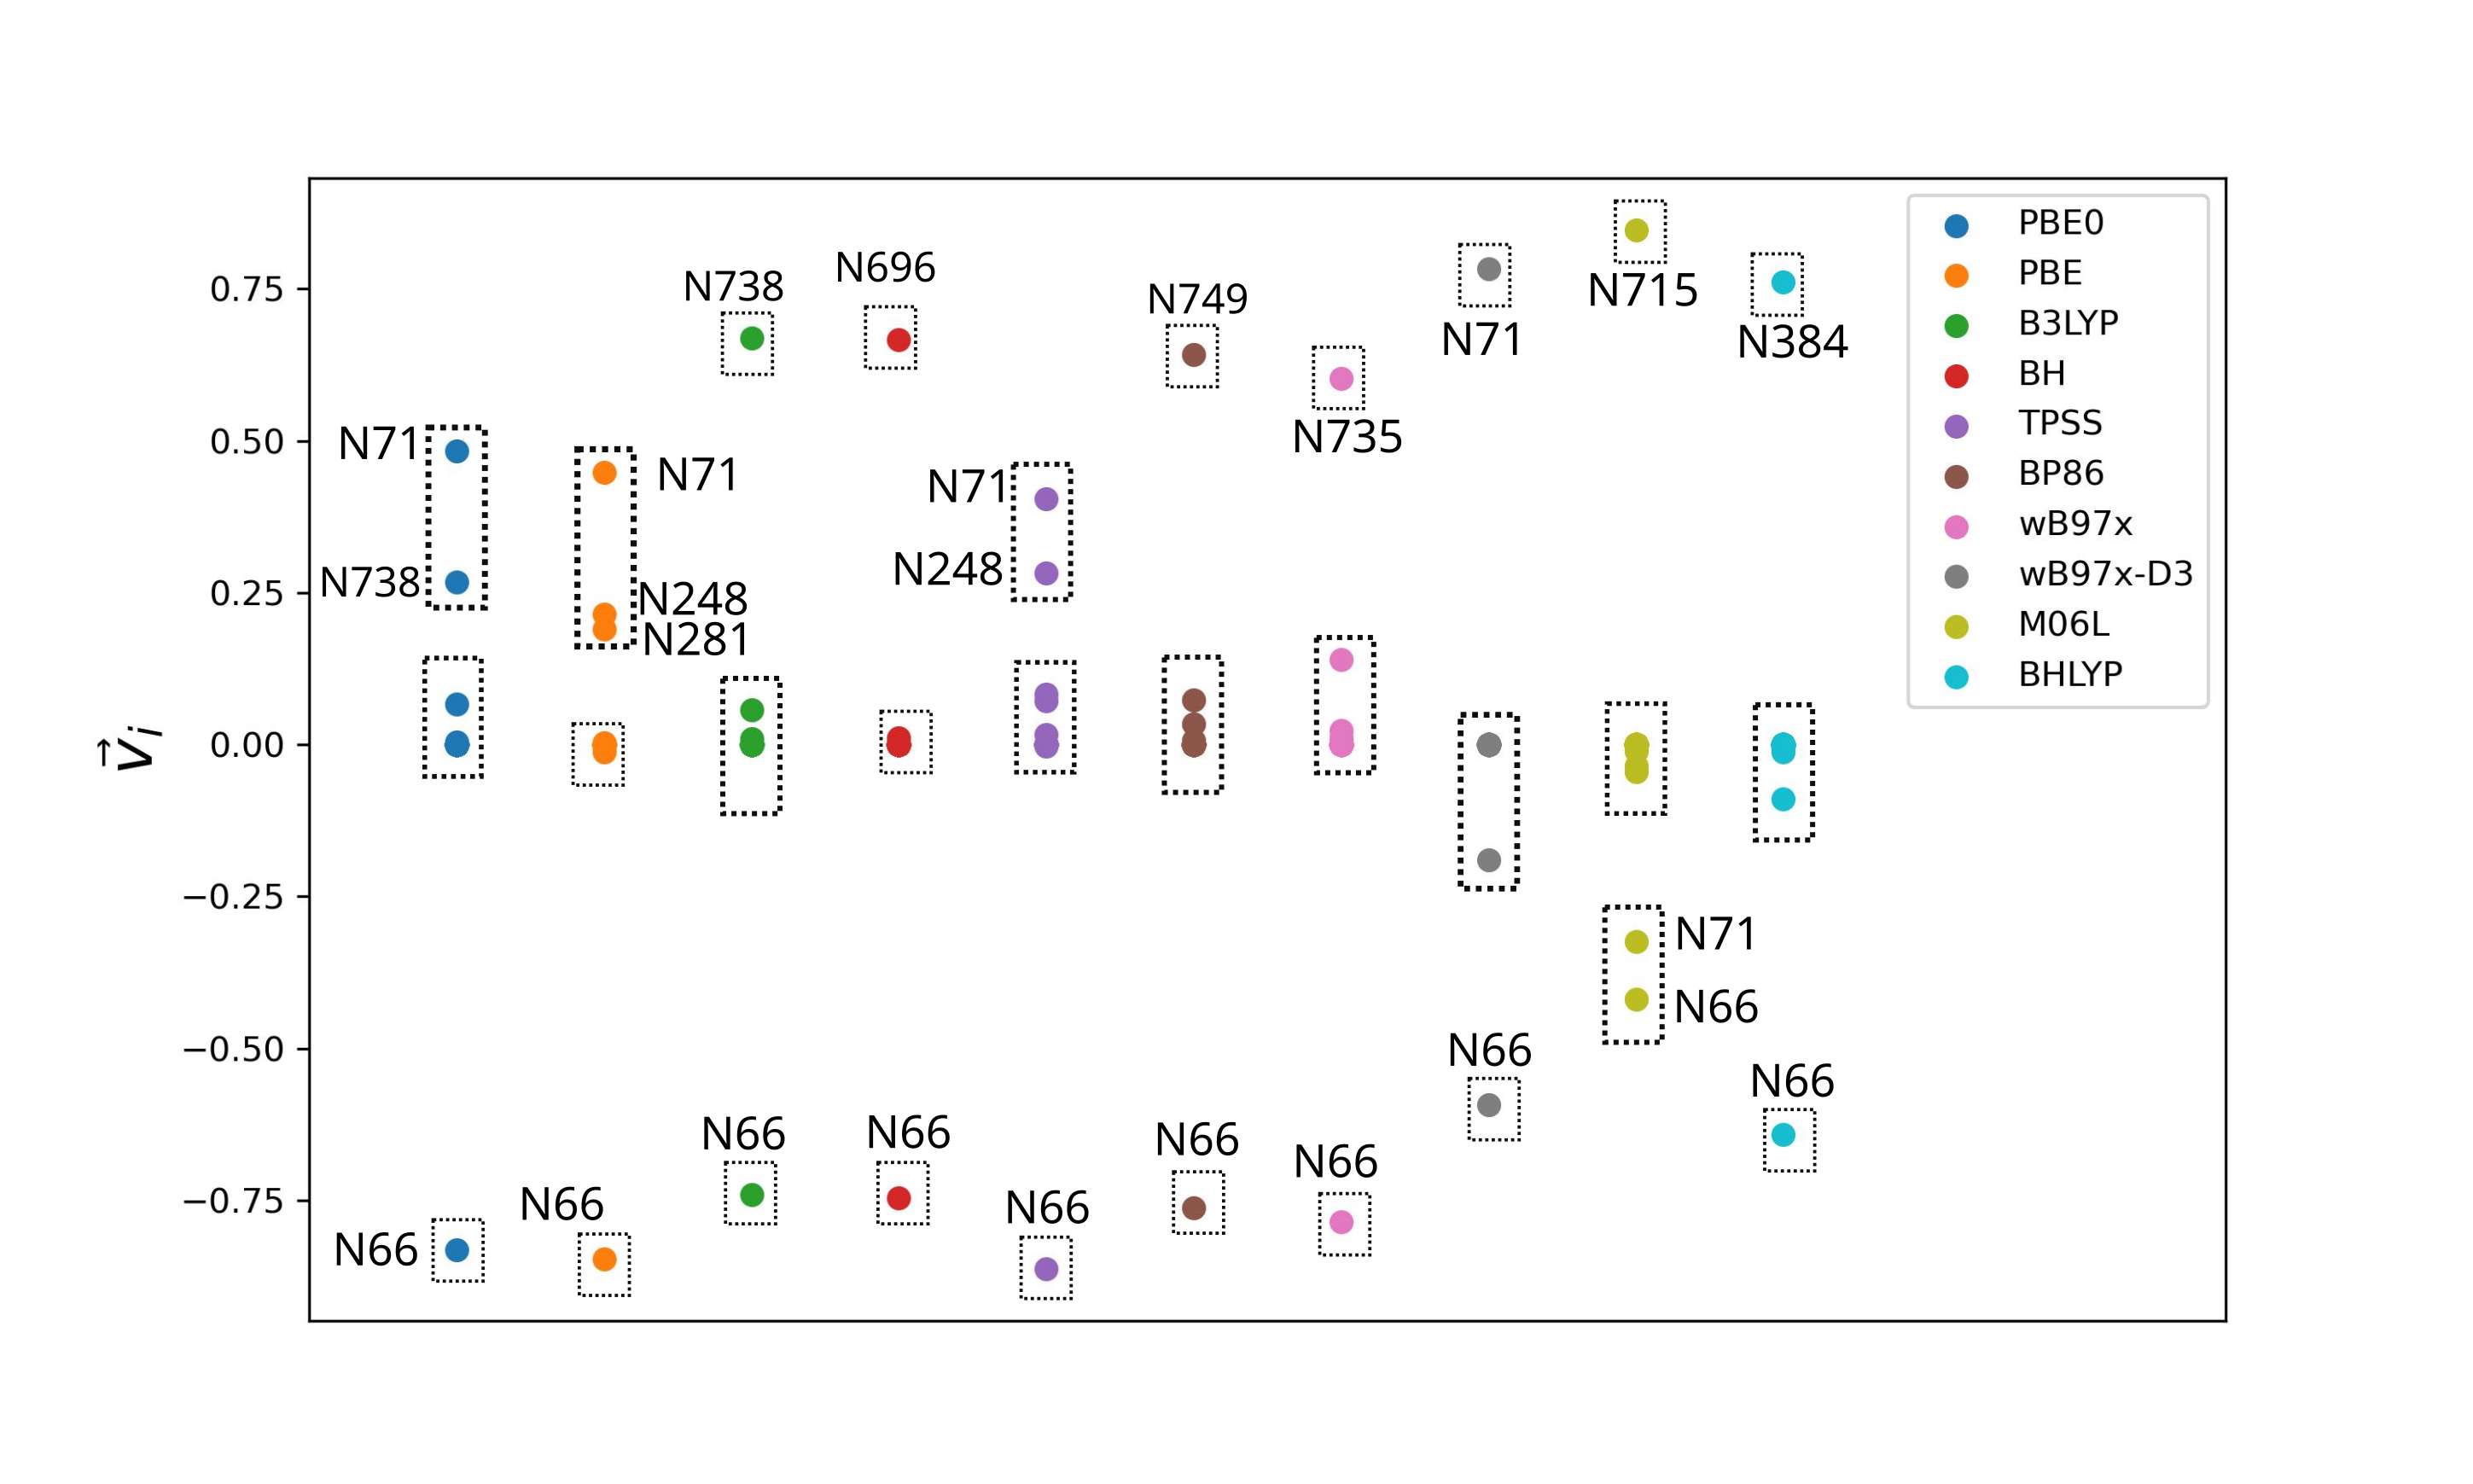
\includegraphics[width=0.8\textwidth]{figs/fig_2ndVecLw.png}
    \caption{Scatter plot of the eigen vector entries $\Vec{v}_i$ of $L_W$ for various $f$ indicated by the legend and point color. 
    The numbers are node index. The dash rectangular indicates the 3-means clusters that are detected as clusters by the Kmeans Lloyd's algorithm. }
    \label{fig:2ndVecLW}
\end{figure}

\begin{figure}
    \centering
    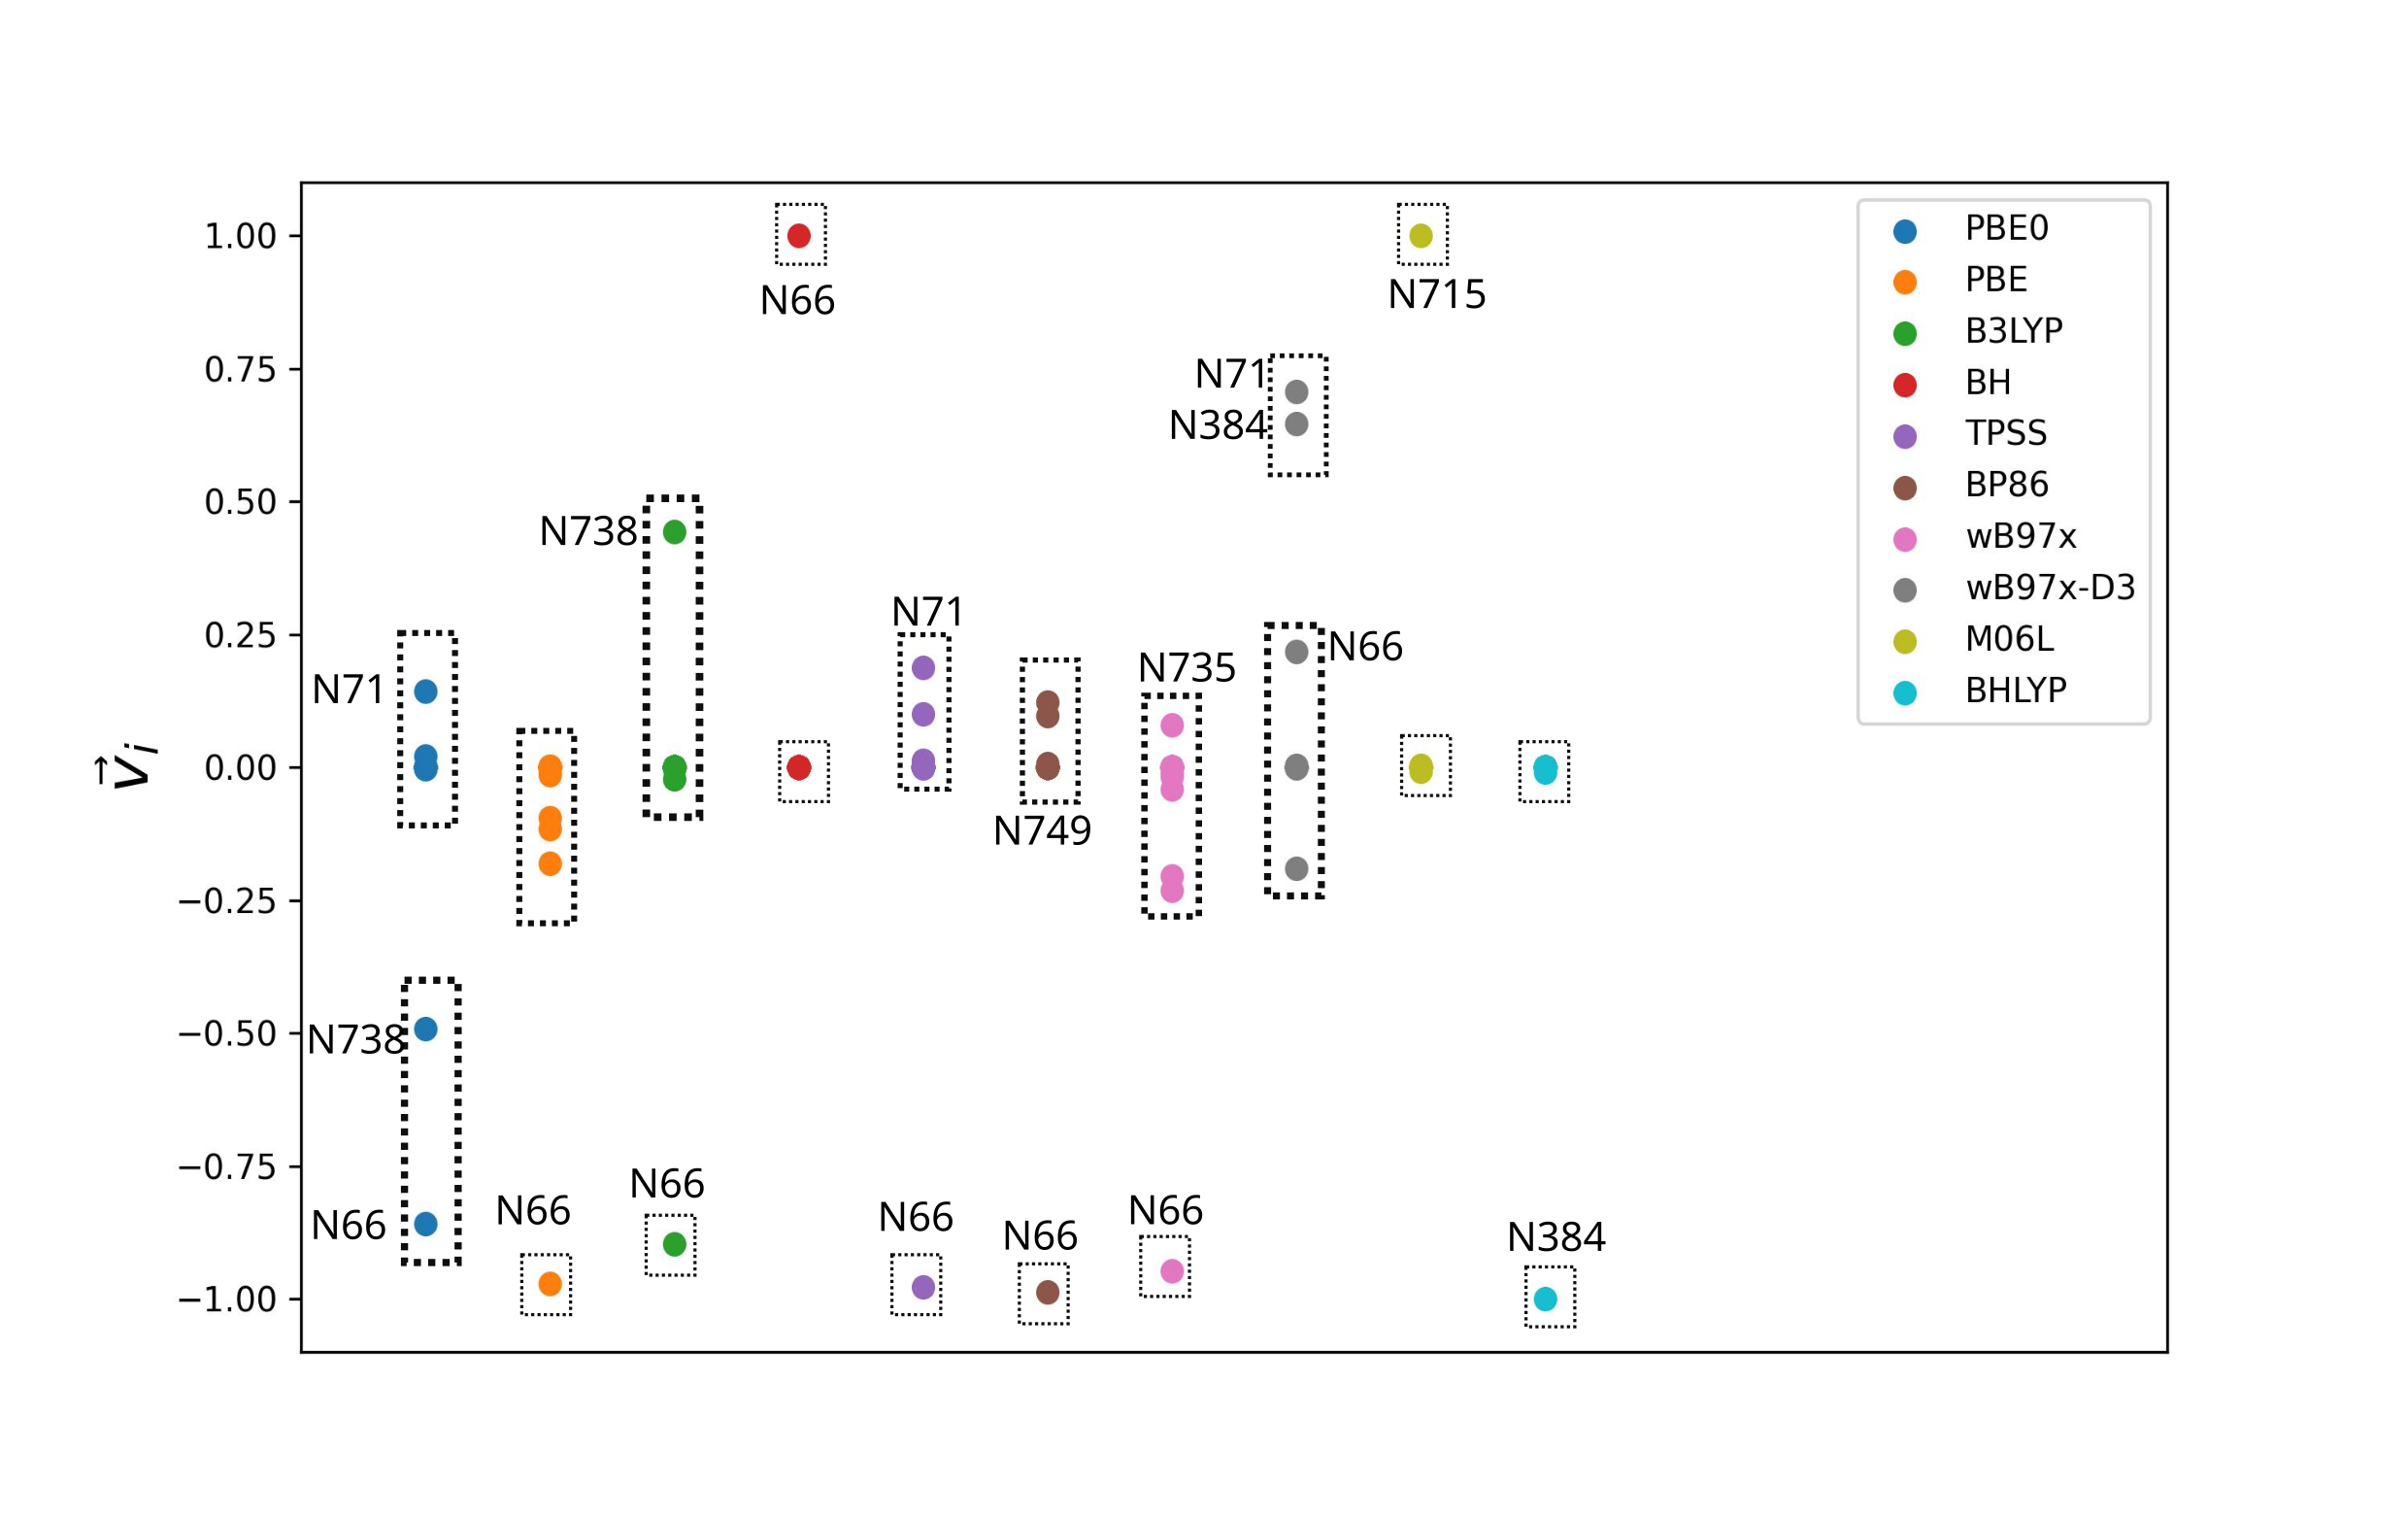
\includegraphics[width=0.8\textwidth]{figs/fig_2ndVecRW.png}
    \caption{Scatter plot of the eigen vector entries $\Vec{v}_i$ of $L_{rw}$ for various $f$ indicated by the legend and point color. 
    The numbers are node index. The dash rectangular indicates the 3-means clusters that are detected as clusters by the Kmeans Lloyd's algorithm.  }
    \label{fig:2ndVecRW}
\end{figure}

From Figs. \ref{fig:2ndVecLW} and \ref{fig:2ndVecRW}, certain nodes, such as node 66, are isolated from most of the graph. The distributions of the second eigenvector entries reveal that a few points are separated from the rest. For example, both figures show that node 66 is often partitioned as a cluster where the CTMC spends significant time compared to other nodes. Since those distributions show similar structure, we need to have an indicator to find out which nodes slow the dynamics.

Recalling that the second eigenvalue is a metric derived from graph partitioning while the second eigenvector contains the entries, we further find that the cost function $Z$ from K-means clustering is correlated with the ToF. Scatter plots of $Z$ and ToF are shown in Fig. \ref{fig:fig_Z_ToF}. K-means clustering requires the number of clusters as input, determined using the kernel density estimation (KDE) method described in the Appendix.

Figure \ref{fig:fig_Z_ToF} shows scatter plots of K-means clustering partition cost $Z_{2c}, Z_{3c}$ versus ToF. For the normal Laplacian $L_w$, $Z_{2c}$ is not correlated with the ToF, but $Z_{3c}$ is. For the Random-walk Laplacian, both $Z_{2c}$ and $Z_{3c}$ show a strong correlation with ToF. Thus, the clustering cost function indicates the speed of charge dynamics as measured by ToF.

\begin{figure}
    \centering
    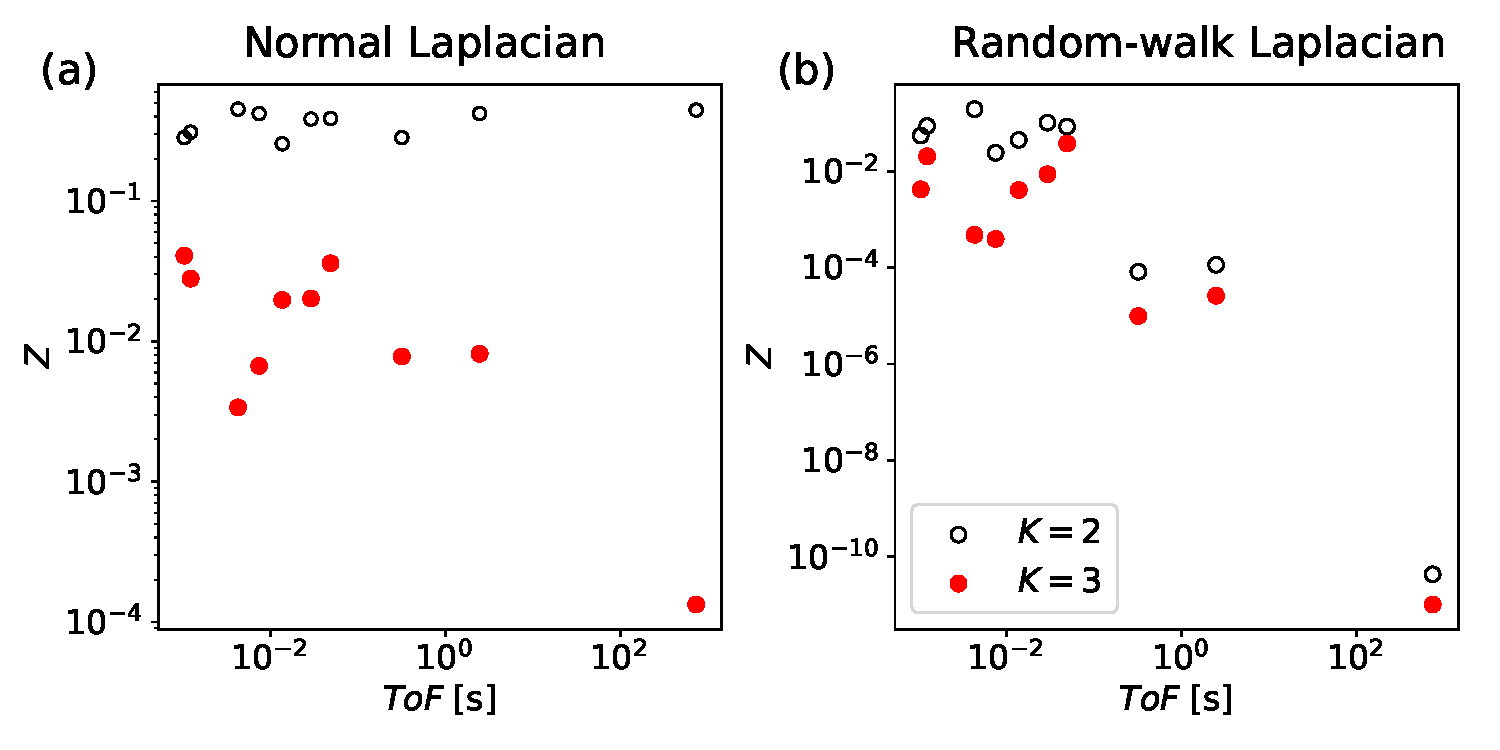
\includegraphics[width=0.9\textwidth]{figs/fig_Z_ToF.pdf}
    \caption{Scatter plot of $Z$ vs $\text{ToF}$. (a): K-means partition of the second eigenvector of $L_W$ for $K=2$ and $K=3$ (b) K-means partition of the second eigenvector of $L_{RW}$ for $K=2$ and $K=3$}
    \label{fig:fig_Z_ToF}
\end{figure} 

\subsection{Trap energy effect and cost function}
As shown in Figs. \ref{fig:2ndVecRW} and \ref{fig:fig_Z_ToF}, $Z$ can identify nodes/molecules (traps) that cause large ToF. However, we need to clarify how a single trap energy $E_t$ affects $Z$ before using $Z$ to identify traps. Specifically, we need to determine the sensitivity of $Z$ to the trap energy $E_t$ and ToF, and the functional form of $Z(E_t)$.

To investigate the effect of trap energy on $Z$, we vary $E_t$ in the PBE functional system over a range from small to large values: $[-2.0, -0.3]$. Node 66 is chosen as the trap. We then calculate the ToF and $Z$ from 2-means clustering with $L_{rw}$.

\begin{figure}
    \centering
    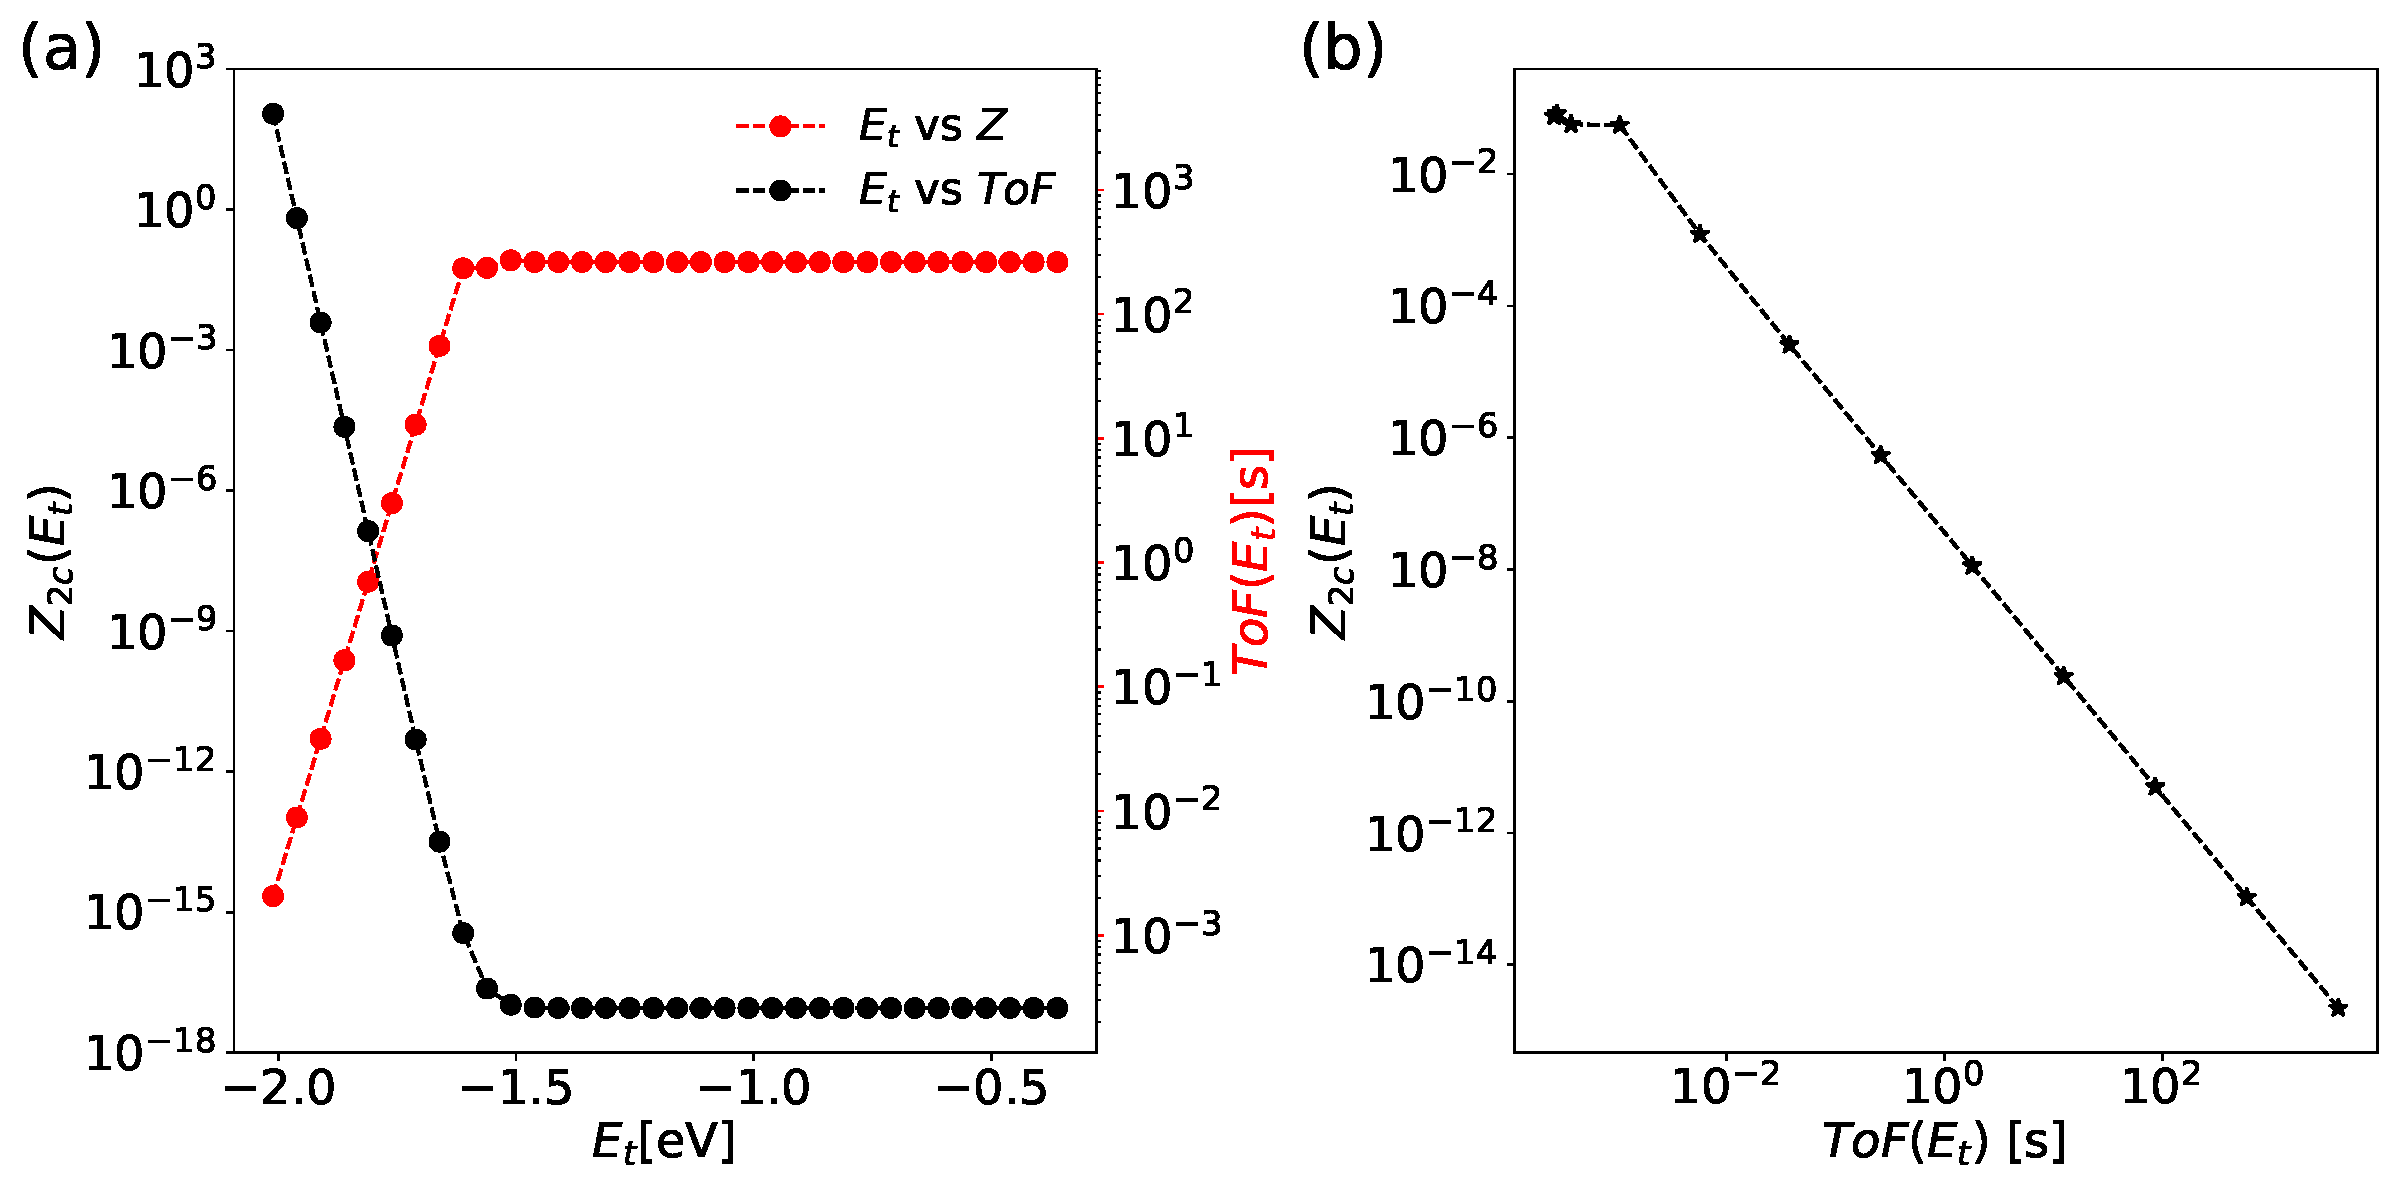
\includegraphics[width=0.8\textwidth]{figs/fig_E_ToF_Z_nonsym.pdf}
    \caption{Scatter plot of $E_t$ vs $Z$, and ToF vs $Z$ for the BCP system with PBE functionals.}
    \label{fig:fig_E_ToF_Z2_Lrw}
\end{figure}

Figure \ref{fig:fig_E_ToF_Z2_Lrw} shows a linear relationship between $E_t$ and $\log_{10} Z$ when $E_t < -1.6$. As $E_t$ increases, node 66 is no longer identified as a cluster because it is rarely visited in the CTMC. When $E_t$ is very large, both the out-going and in-going rates are small, but the in-going rate is much smaller. The ToF vs. $\log_{10} Z$ plot shows that ToF remains unchanged as $E_t$ continues to increase.

Thus, spectral clustering using $\vec{v}_2$ of $L_{rw}$ can identify traps in the system but cannot detect nodes that are rarely visited (anti-traps).



To identify anti-trap nodes using spectral clustering, we symmetrize the adjacency matrix:
\begin{equation}
    W := \frac{1}{2}(W + W^T)
\end{equation}
and use the second eigenvector $\vec{v}_2$ of $L_\text{sym} = \text{diag}(W) - W$, where $\text{diag}(W)$ is the out-degree matrix of $W$. We then calculate the cost function $Z$.

The relationship between the cost function from $L_\text{sym}$ and $E_t$ is shown in Fig.\ref{fig:fig_E_ToF_Z2_1}.

\begin{figure}
    \centering
    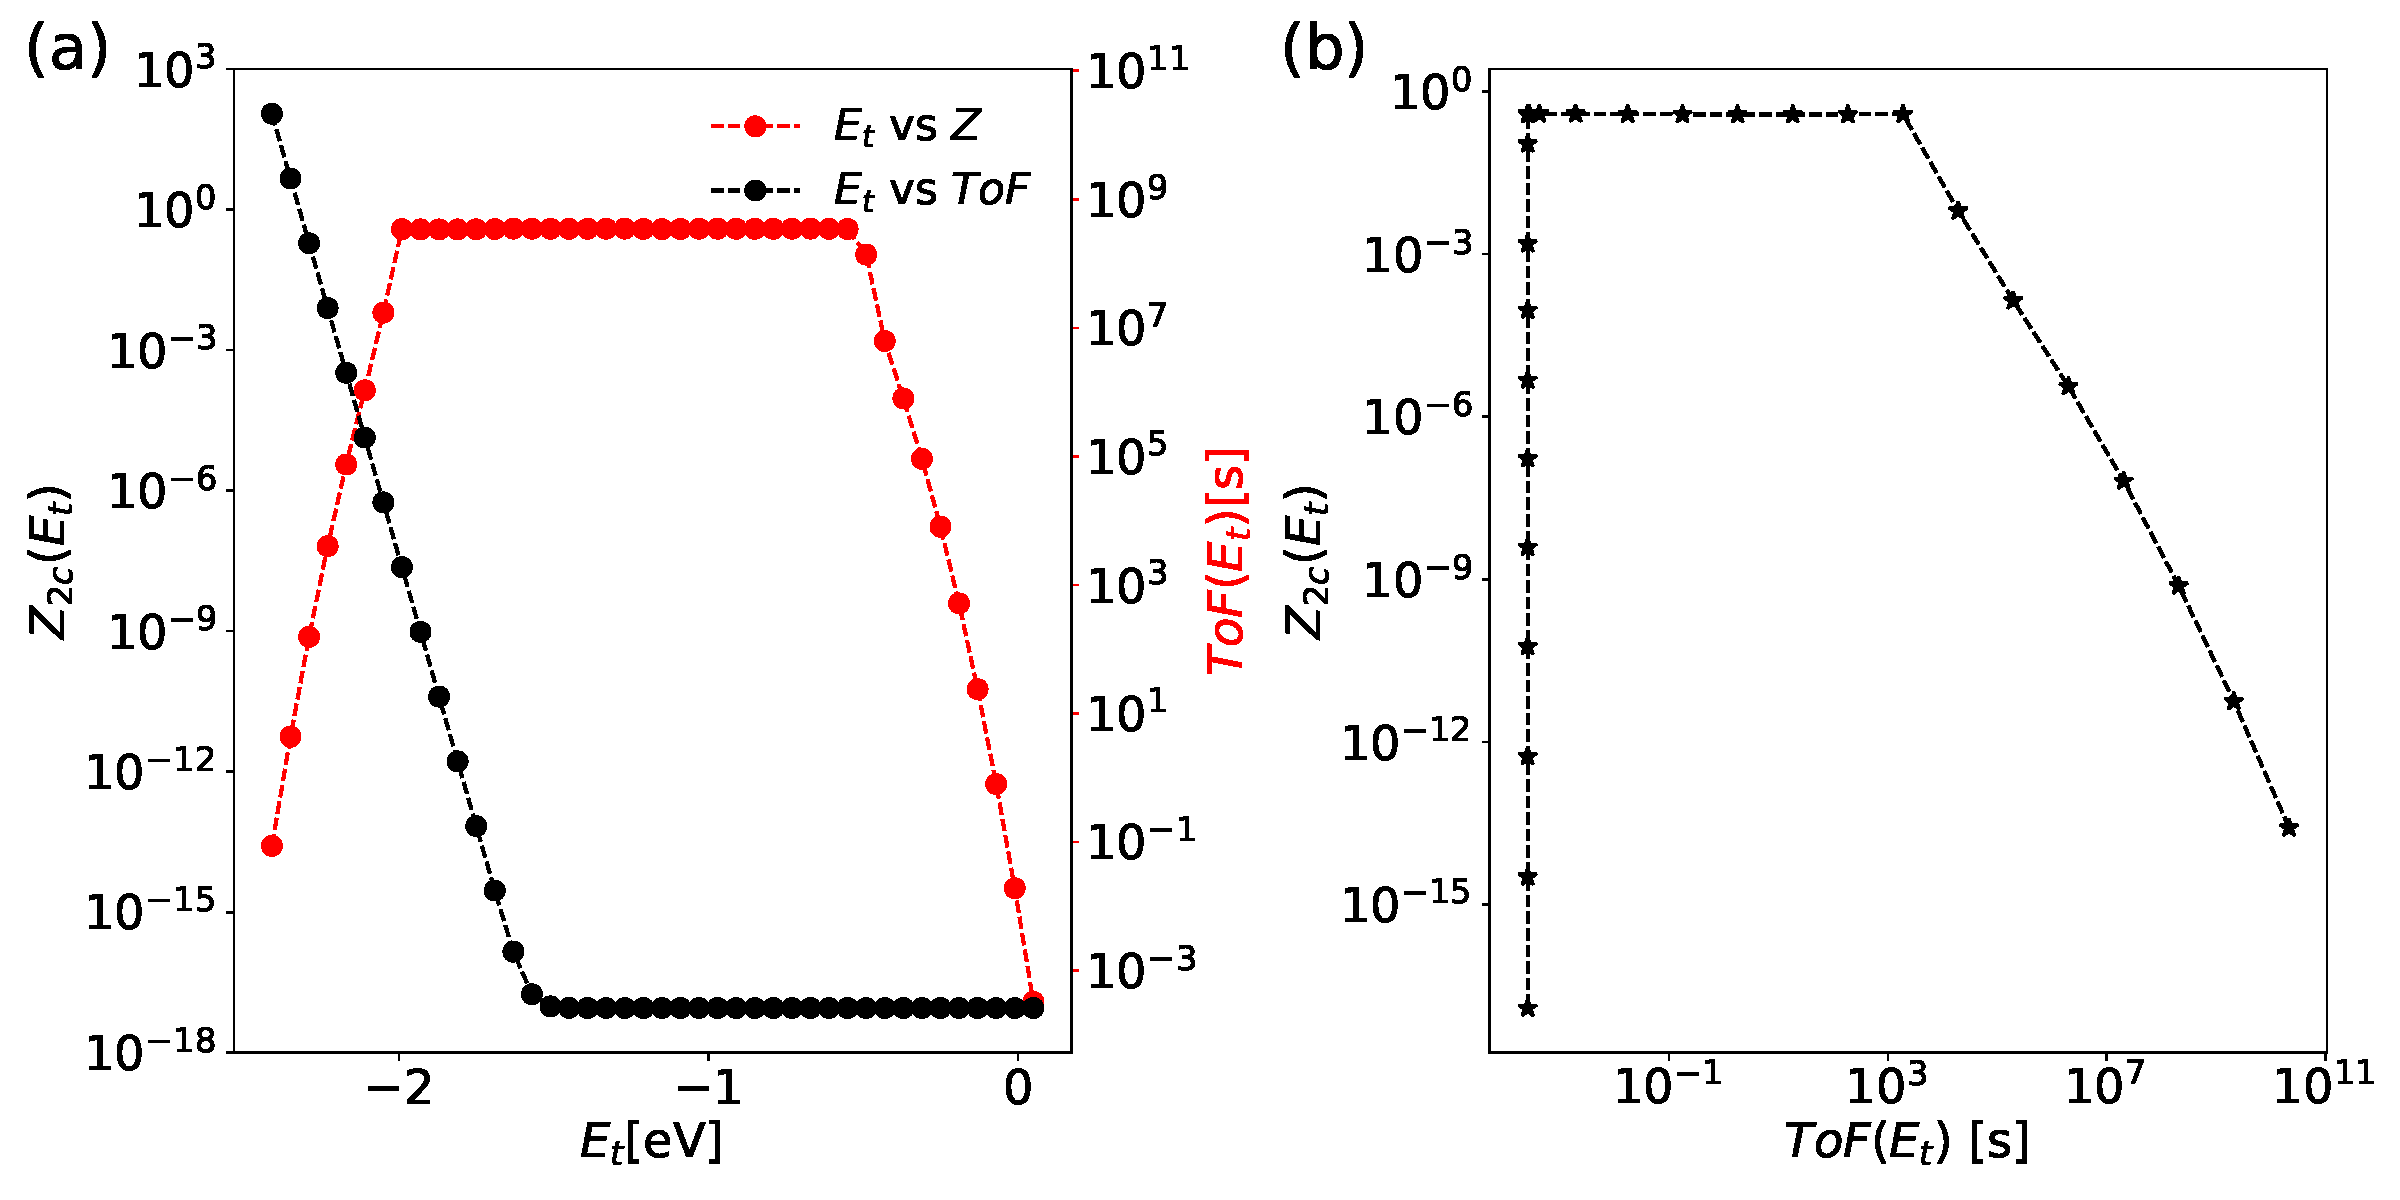
\includegraphics[width=0.8\textwidth]{figs/fig_E_ToF_Z_sym.pdf}
    \caption{Scatter plot of $E_{66}$ vs $Z$, and ToF vs $Z$ for the BCP system with PBE functionals. The cost function $Z$ is calculated from 2-means clustering on the $\vec{v}_2$ of $L_\text{sym}$.}
    \label{fig:fig_E_ToF_Z2_1}
\end{figure}

When $E_t$ is very small ($<-2$), node 66 is identified as a separate cluster, and $Z$ decreases as $E_t$ decreases, while ToF increases. 

For $-0.5 > E_t > -2.0$, $Z$ remains relatively stable since other nodes can be identified as a second cluster. When $E_t > -0.4$, node 66 is again identified as a cluster, and $Z$ decreases as $E_t$ increases. However, ToF remains unchanged because a high $E_t$ results in the node being rarely visited.
Partitioning $\vec{v}_2$ of $L_\text{sym}$ when $E_t$ is not too low will not identify node 66 as a trap cluster, unlike $\vec{v}_2$ of $L_{rw}$ or $L_{W}$, as seen in the BHANDHLYP functional BCP system. This is because the in-going rate from neighbors to node 66 is not small compared to other rates, although the out-going rate is small. Using $L_\text{sym}$ averages the edge weights, making $W_{66,i}$ larger. Therefore, $\vec{v}_2$ of $L_\text{sym}$ will not identify node 66 as a separate cluster in the BHANDHLYP system.

In conclusion, $\vec{v}_2$ of $L_\text{sym}$ can identify both traps and anti-traps only when both in-going and out-going rates are small compared to all rates.

\section{Conclusion}
\label{sec:con}

In this study, we investigated the influence of various functionals on the electronic properties and time-of-flight in charge transport systems. Our multiscale model demonstrated that different exchange-correlation functionals can significantly impact ToF although the electronic parameters such as the reorganization energy, energy disorder, and mobility do not change significantly.
Through extensive analysis, including scatter plots and clustering, we identified that certain nodes exhibit distinct behaviors, forming clusters that correlate with ToF variations.

Key findings include the identification of a log-linear relationship between clustering partition cost and ToF under varying conditions, particularly highlighting role of the trap energy $E_t$ effect. 
Additionally, the use of the random walk Laplacian matrix and symmetrized Laplacian matrix allowed us to identify both trap and anti-trap nodes effectively depending on $E_t$ scale, correlating well with partition cost metrics. 

In summary, this study provides a comprehensive analysis of how electronic properties influence charge transport, offering valuable insights for future research in optimizing functional selection for accurate ToF predictions in electronic systems.




\section{Appendix}
\label{sec:stat}
To investigate the distribution of parameters and quantity of interest, correlation functions and distribution distance need to be used. 

\subsection{Correlation Coefficient}
The Spearman rank correlation coefficient, denoted as $\rho$, a statistical measure of the strength and direction of association between two ranked variables, is used to quantify the correlation between two sets of variables:
\begin{equation}
\rho = 1 - \frac{6 \sum d_i^2}{n(n^2 - 1)}    
\end{equation}
where $d_i$ is the difference between the ranks of corresponding pairs of observations, and
$n$ is the number of observations.

A value of 1 indicates a perfect positive monotonic relationship, where high ranks of one variable are consistently associated with high ranks of the other, and vice versa.
A value of -1 indicates a perfect negative monotonic relationship, where high ranks of one variable are associated with low ranks of the other, and vice versa.
A value of 0 suggests no monotonic relationship between the variables.

Spearman's $\rho$ is used because it makes fewer assumptions about the underlying distribution of the data compared to Pearson's correlation coefficient. It does not assume that there is a linear relationship between variables. 
It measures the strength of monotonic relationships between variables, meaning it captures whether variables tend to increase or decrease together, even if the relationship is not strictly linear. This makes it particularly useful when assessing associations in data where the relationship may be nonlinear or when the variables have a consistent direction of change but not necessarily a linear one.


\subsection{Distance between Two Distributions}
Let $P_1$,$P_2$ be two distributions with probability density $p_1,p_2$. 
There are many ways to define a distance between P and Q such as:
Total variation: $\frac{1}{2}\int |p_1 - p_2|$, $L_2$ distance $\int |p_1 - p_2|^2$, Hellinger: $\sqrt{\int (\sqrt{p_1}-\sqrt{p_2})^2}$, Kullback-Leibler Divergence\cite{csiszar_divergence_1975} and Wasserstein distance\cite{villani_optimal_2009}.

For a $S \in \mathcal{S}$, the vector $\Vec{E}_f$ can be seen as a collection of $N$ random variables, its empirical cumulative distribution function can be written as:
$P_f(E) = \frac{1}{N} \sum\limits_{i=1}^N U(E-E_i)$ where $U(x)$ is the unit-step function with $U(0) = 0.5$. 

We choose to use Kullback-Leibler (KL) divergence and Wasserstein distance instead of Total variation, $L_2$ distance and Hellinger 
because these distances ignore the underlying geometry of the space, and they can not be used to compare $P_1$ and $P_2$ when one is discrete and the other is continuous.

The KL Divergence quantifies how difficult it is to discriminate between two populations with the best test\cite{csiszar_divergence_1975}, its estimator is given by\cite{noauthor_2008_2008}:
\begin{equation}
    \Hat{D}(P_f||P_{f'}) = \frac{1}{N} \sum\limits_{i=1}^N \log \frac{\delta P_f(E_i)}{\delta P_{f'}(E_i)}
\end{equation}
where $\delta P_f(E_i) = P_f(E_i) - P_f(E_i - \epsilon) $ for any $\epsilon < \min_i \{ E_i - E_{i-1} \}$.

The Wasserstein distance for two empirical distributions $P$ of dataset $X_1,\cdots,X_n$ and $Q$ of dataset $Y_1, Y_2,\cdots, Y_n$ can be computed using:
\begin{equation}
    W_p (P,Q) = (\sum_i || X_i - Y_i ||^p )^{\frac{1}{p}}
\end{equation}
If the dimension of the dataset $d>1$,  then
\begin{equation}
    W_p (P,Q) = \inf_{\pi} (\sum_i || X_i - Y_i ||^p )^{\frac{1}{p}}
\end{equation}
where the infimum is over all permutations $\pi$. 

There are differences between Wasserstein distance and KL Divergence.
Wasserstein distance defines a metric on the space of probability distributions, meaning it satisfies properties like non-negativity, symmetry, and the triangle inequality. This makes it useful for clustering, classification, and optimization problems where a notion of distance or similarity between distributions is required. KL divergence, on the other hand, is not a metric as it lacks symmetry and the triangle inequality.
Wasserstein distance tends to be more stable under small perturbations in the distributions compared to KL divergence. This can be advantageous in situations where the data is noisy or uncertain. For completeness, we use both Wasserstein distance and KL divergence to measure the distribution distance.

\subsection{KDE Method of Finding Cluster Number}
For 1D clustering problem kernel density estimation (KDE) is often used to find the number of clusters that correspond to peaks of eigenvector elements. 
Let $(x_1, x_2, \cdots, x_n)$ be independent and identically distributed samples drawn from some univariate distribution with an unknown density $f$ at any given point $x$.
The kernel density estimator is:
\begin{equation}
    \hat{f}_h(x) = \frac{1}{nh} \sum\limits_{i=1}^n K(\frac{x-x_i}{h})
\end{equation}
Where $K(x) = \frac{1}{\sqrt{2\pi} } e^{-\frac{1}{2}x^2}$ is the kernal and here the standard normal density function is used, $h$ is a smoothing parameter which influences the smoothness and accuracy of the estimated density. An optimal choice\cite{silverman_density_1998} is $h=(\frac{4 \sigma^5}{3n})^{1/5}$ where $\sigma$ is the sample standard deviation and $n$ the sample size.

The kernel density estimator plot is shown in Fig.\ref{fig:kde}. This figure shows that, in the systems where two-cluster partitions have a large $Z$ cost function, it can be further subdivided into smaller clusters. 

The peaks correspond to the scatter groups in Fig.\ref{fig:d_eig_tof3}. 

\begin{figure}
    \centering
    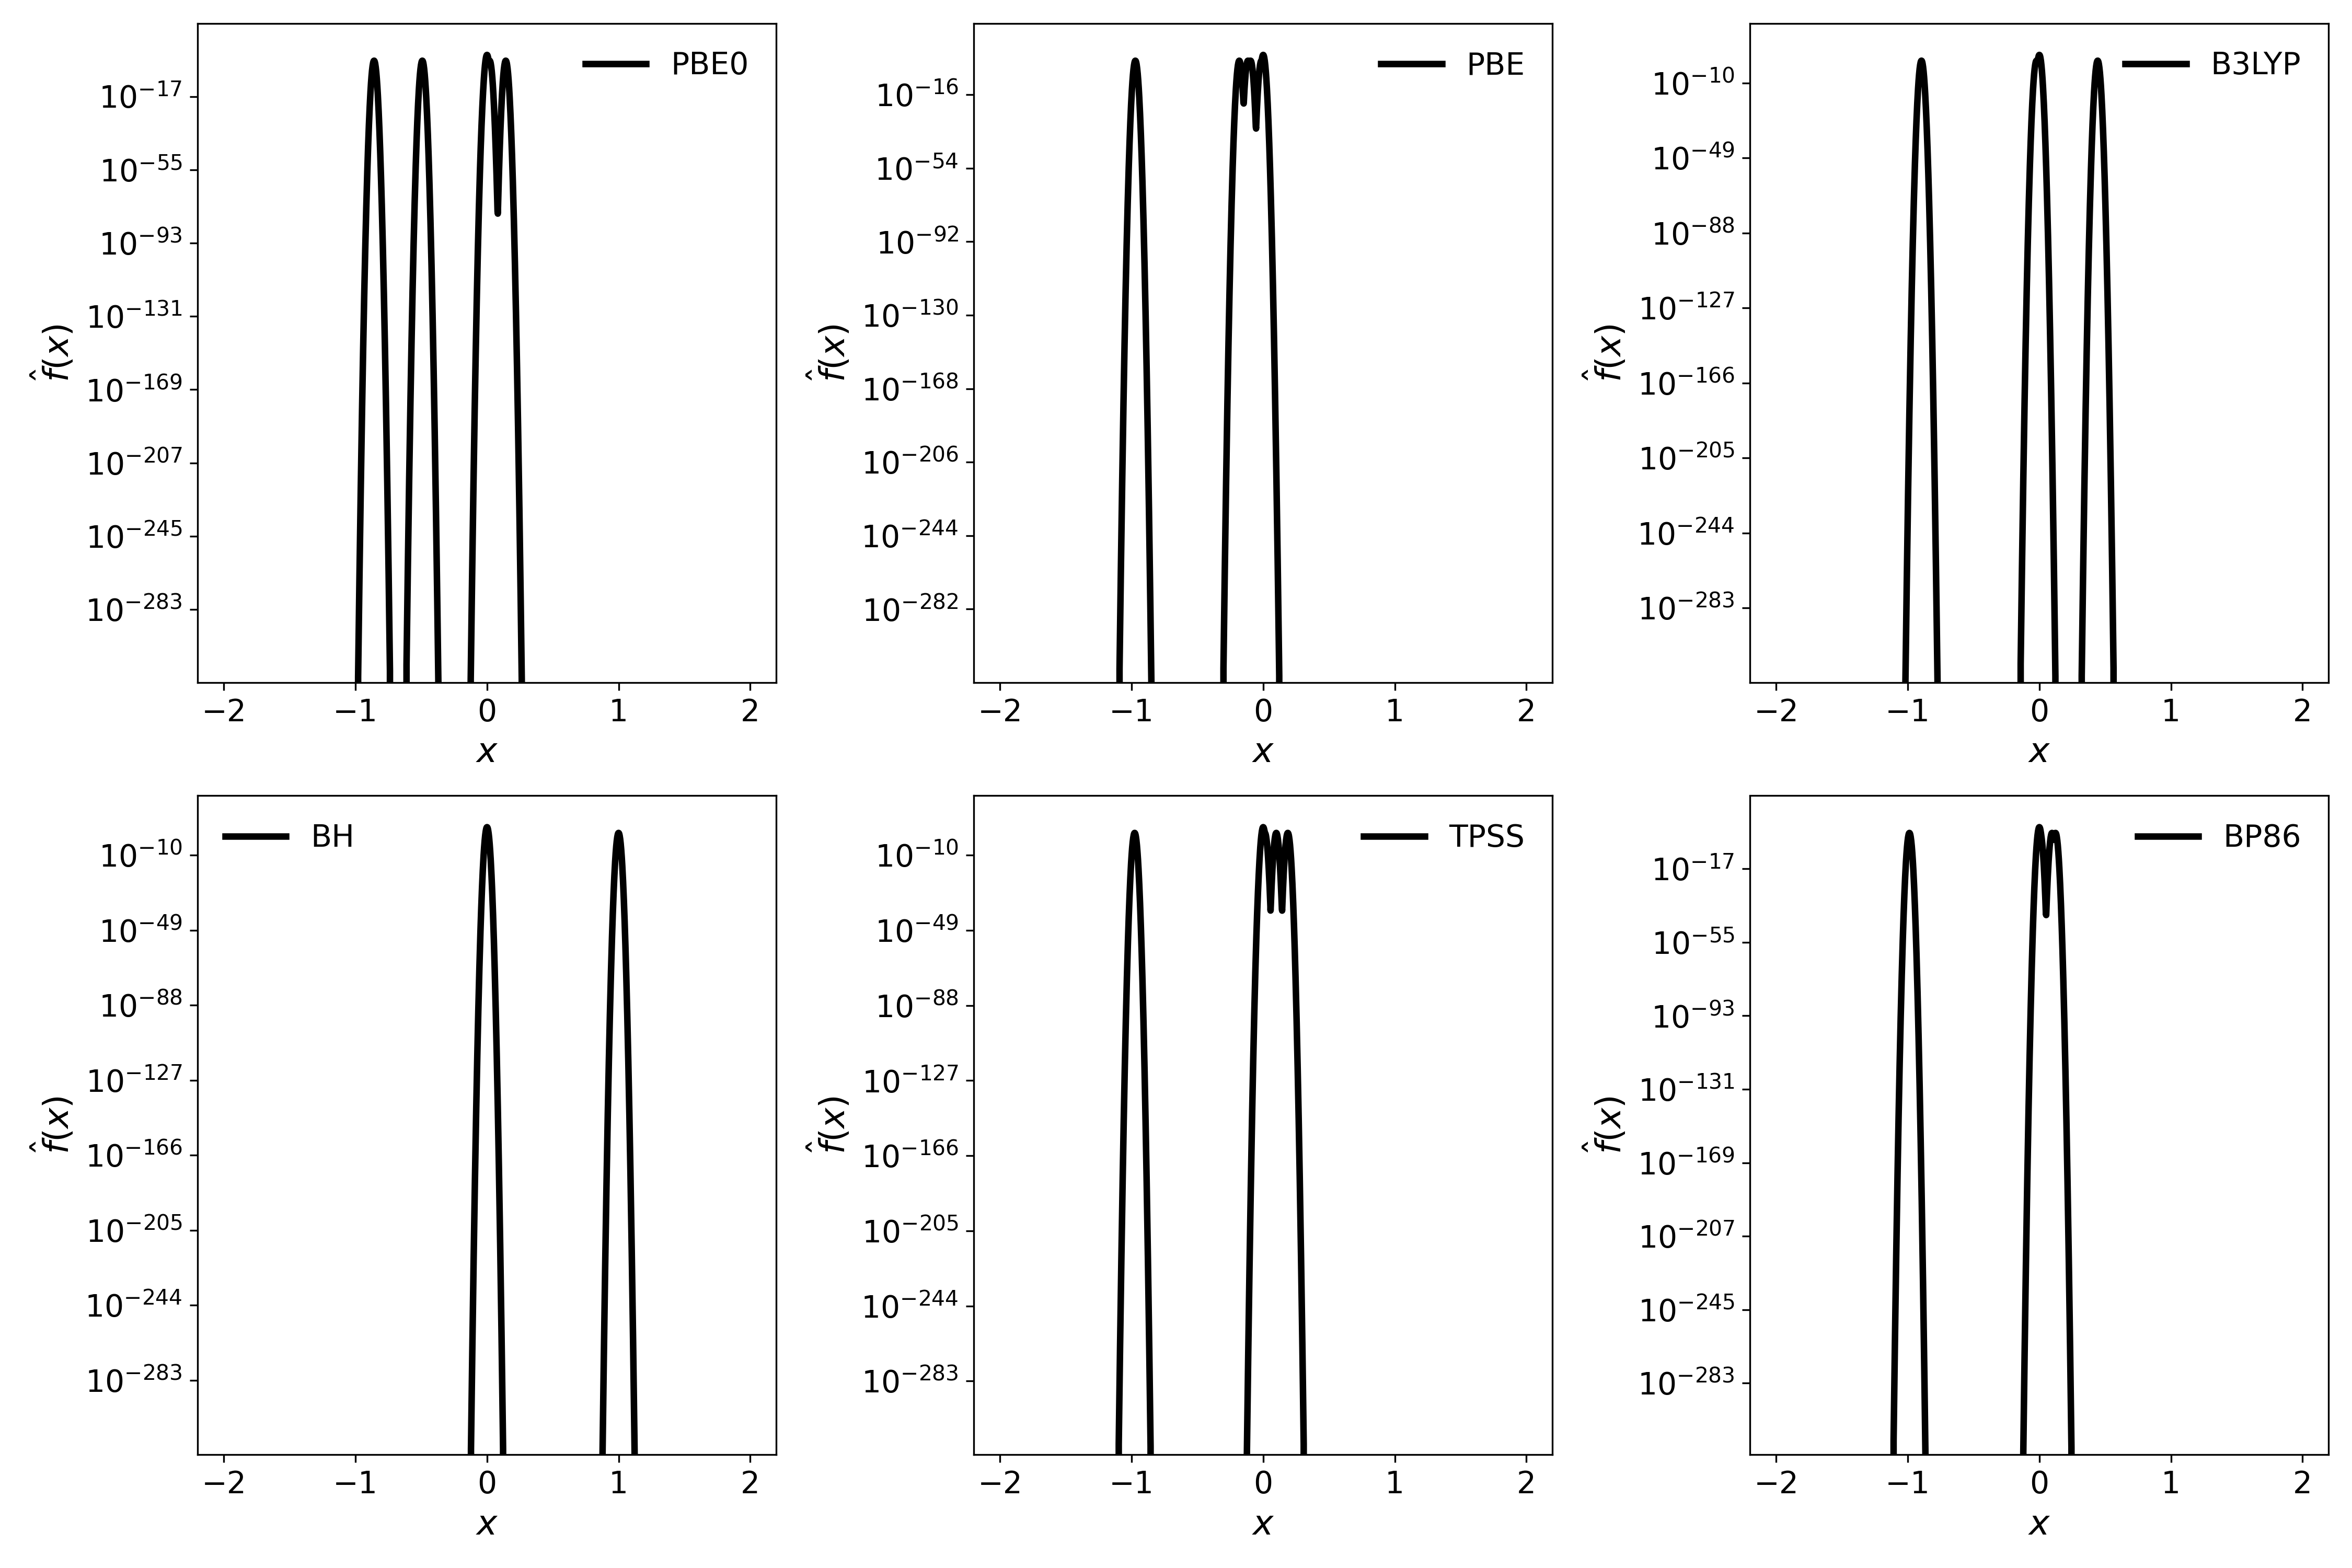
\includegraphics[width=1.0\textwidth]{figs/kde.png}
    \caption{$\hat{f}_h(x)$ as a function of $x$ with $h=1e-5$. In each plot Y-axis represents $\hat{f}_h(x)$ and X-axis represents $x$. The legend indicates the functionals.}
    \label{fig:kde}
\end{figure}

\subsection{Other Parameter Difference and ToF Difference}
\begin{figure}
    \centering
    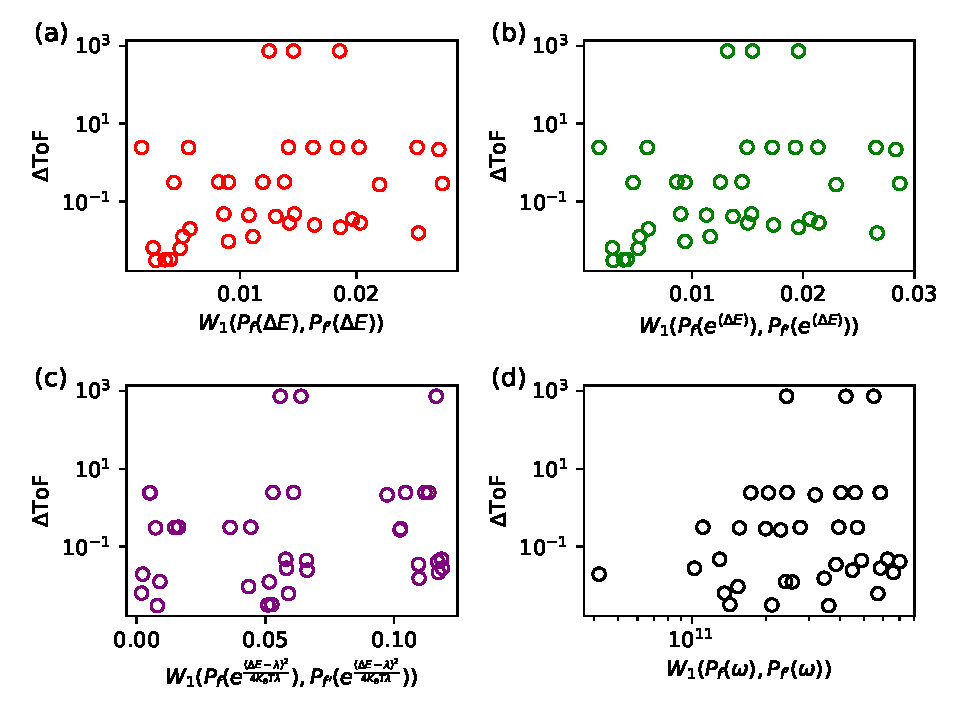
\includegraphics[width=0.7\textwidth]{figs/DeltaToF_W_all.pdf}
    \caption{Scatter plot of (a): $W_1(P_f(\Delta E),P_{f'}(\Delta E))$, (b): $W_1(P_f(\exp(\Delta E)),P_{f'}(\exp(\Delta E)))$, (c): $W_1(P_f(\exp \frac{-(\Delta E - \lambda)^2}{4 k_B T \lambda}),P_{f'}(\exp \frac{-(\Delta E - \lambda)^2}{4 k_B T \lambda}))$ and (d): $W_1 (P_f(\omega), P_{f'}(\omega) )$ vs. $\Delta \text{ToF}$.   }
    \label{fig:d_WD_tof}
\end{figure}
Fig. \ref{fig:d_WD_tof} explores $\Delta \text{ToF}$ relative to properties derived from the energy distribution ($\Delta E$) and related transformations, revealing that while the Wasserstein distance remains stable across different functionals, $\Delta \text{ToF}$ varies notably.

\begin{figure}
    \centering
    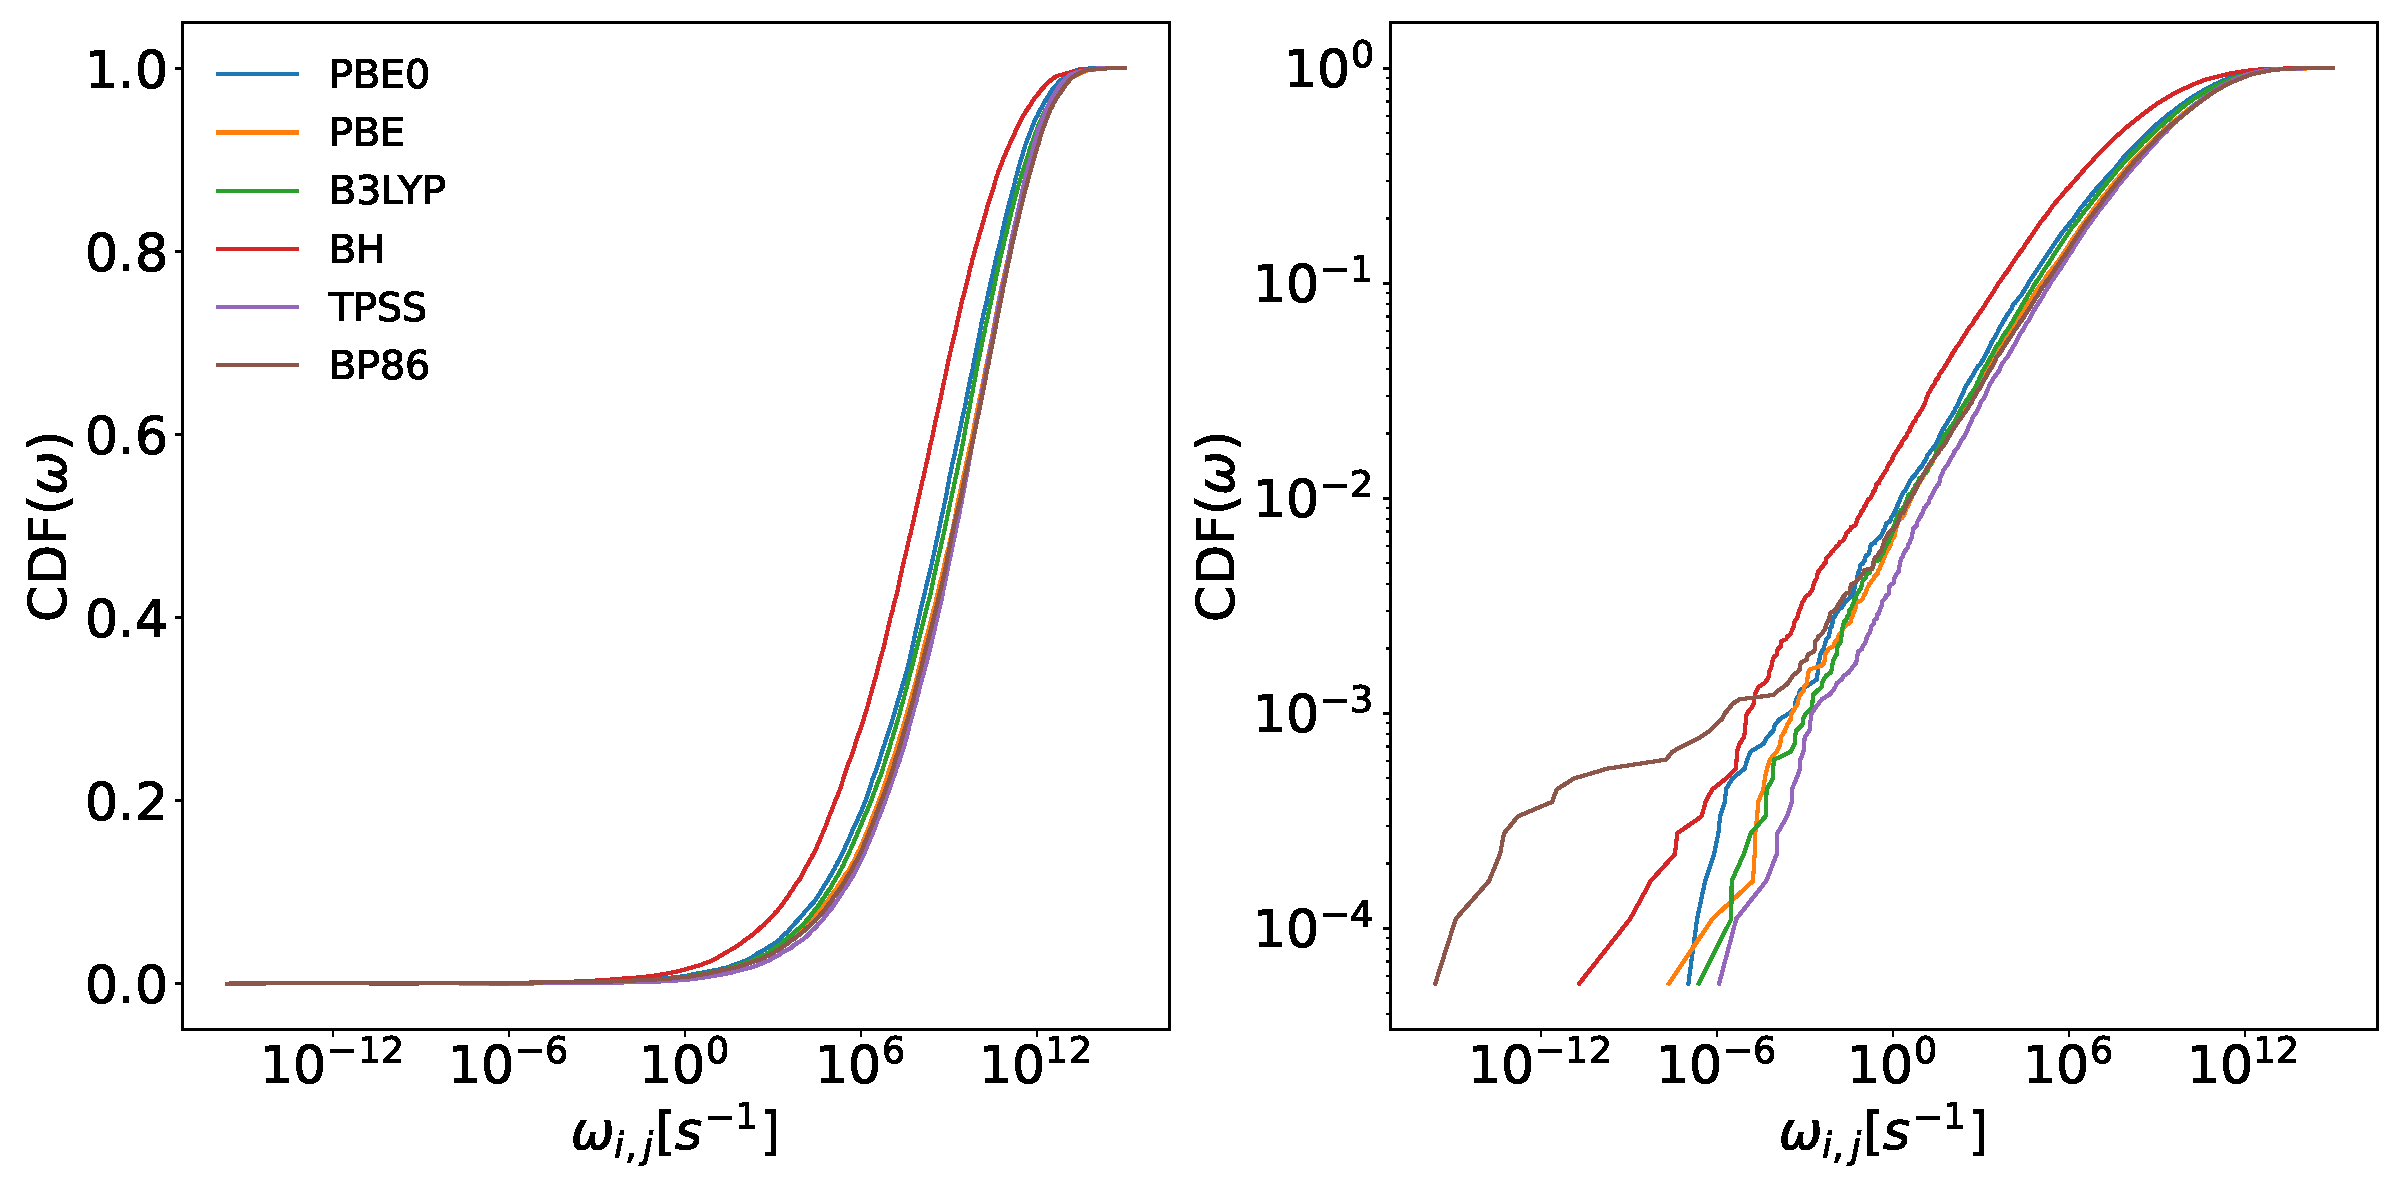
\includegraphics[width=0.9\textwidth]{figs/cdf_w_log.pdf}
    \caption{Empirical distribution of Marcus rates in the seven systems whose function is indicated by the legend. Left: no log scale, right: with log scale}
    \label{fig:cdf_w}
\end{figure}
Fig. \ref{fig:cdf_w} depicts the empirical cumulative distribution function of Marcus rates calculated with different functionals, to find the correlation of $\omega$ with ToF, particularly noting the distinct behavior of the BP86 functional although its ToF is close to that of PBE0. 
So the correlation between $P_f(\omega)$ and ToF is not obvious, and it is delusive to tell how the ToF is correlated to the parameters $E,J_{i,j}$ and $\omega$.

In summary, these findings indicates the nuanced relationship between electronic properties ($E_i$, $J_{i,j}$, $\lambda_{i,j}$) and $\omega$, and eventually the ToF in  charge transport systems. 

\bibliographystyle{unsrt}
\bibliography{references}

\end{document}
